%description: Mathematical Article in English (AMS)
%% Based on a TeXnicCenter-Template by Gyorgy SZEIDL.
%% Used as a template by Mohsin Javed
%% Sep 29, 2017
%%%%%%%%%%%%%%%%%%%%%%%%%%%%%%%%%%%%%%%%%%%%%%%%%%%%%%%%%%%%%



%------------------------------------------------------------
%
\documentclass{amsart}
%
%----------------------------------------------------------
% This is a sample document for the AMS LaTeX Article Class
% Class options
%        -- Point size:  8pt, 9pt, 10pt (default), 11pt, 12pt
%        -- Paper size:  letterpaper(default), a4paper
%        -- Orientation: portrait(default), landscape
%        -- Print size:  oneside, twoside(default)
%        -- Quality:     final(default), draft
%        -- Title page:  notitlepage, titlepage(default)
%        -- Start chapter on left:
%                        openright(default), openany
%        -- Columns:     onecolumn(default), twocolumn
%        -- Omit extra math features:
%                        nomath
%        -- AMSfonts:    noamsfonts
%        -- PSAMSFonts  (fewer AMSfonts sizes):
%                        psamsfonts
%        -- Equation numbering:
%                        leqno(default), reqno (equation numbers are on the right side)
%        -- Equation centering:
%                        centertags(default), tbtags
%        -- Displayed equations (centered is the default):
%                        fleqn (equations start at the same distance from the right side)
%        -- Electronic journal:
%                        e-only
%------------------------------------------------------------
% For instance the command
%          \documentclass[a4paper,12pt,reqno]{amsart}
% ensures that the paper size is a4, fonts are typeset at the size 12p
% and the equation numbers are on the right side
%
\usepackage{amsmath}%
\usepackage{amsfonts}%
\usepackage{amssymb}%
\usepackage{graphicx}
\usepackage{hyperref}
\usepackage{parskip}


\usepackage{subcaption}



%------------------------------------------------------------
% Theorem like environments
%
\newtheorem{theorem}{Theorem}
\theoremstyle{plain}
\newtheorem{acknowledgement}{Acknowledgement}
\newtheorem{algorithm}{Algorithm}
\newtheorem{axiom}{Axiom}
\newtheorem{case}{Case}
\newtheorem{claim}{Claim}
\newtheorem{conclusion}{Conclusion}
\newtheorem{condition}{Condition}
\newtheorem{conjecture}{Conjecture}
\newtheorem{corollary}{Corollary}
\newtheorem{criterion}{Criterion}
\newtheorem{definition}{Definition}
\newtheorem{example}{Example}
\newtheorem{exercise}{Exercise}
\newtheorem{lemma}{Lemma}
\newtheorem{notation}{Notation}
\newtheorem{problem}{Problem}
\newtheorem{proposition}{Proposition}
\newtheorem{remark}{Remark}
\newtheorem{solution}{Solution}
\newtheorem{summary}{Summary}
\numberwithin{equation}{section}

\DeclareMathOperator*{\argmax}{argmax}

%--------------------------------------------------------
\begin{document}
\title[Quant Finance]{Quantitative Finance in Practice}
\author{Mohsin Javed}
\address[London]
{Pret A Manger, Marble Arch Station, \newline%
\indent Oxford Street, London}%
\email[Mohsin Javed]{mhsnjvd@gmail.com}%
%\urladdr{http://www.zindajaved.com}
%\thanks{This paper is in final form and no version of it will be submitted for
%publication elsewhere.}
\date{September 29, 2017}
%\subjclass{Primary 05C38, 15A15; Secondary 05A15, 15A18} %
%\keywords{Keyword one, keyword two etc.}%
%\dedicatory{Dedicated to ...}

%\begin{abstract}
%\end{abstract}

\maketitle

\section{Introduction}
Mathematical finance, as applied to the 
derivatives market in particular.

\section{Books, Articles and Topics We Should Know}
\begin{itemize}
	\item Black Scholes Model (Read Hull or Shreve)
	\item Change of measure
	\item Change of numeraire
	\item Forward measure
	\item Read Chapter 2 of Brigo/Mercurio
	\item For Quanto/Compo Read paper by Derman on Foreign indices
	\item How is a PDE equivalent to an expectation? (Feynman-Kac and all that)
	\item Forward and backward Kolmograv equations
	\item Local volatility Model (Dupire equation, in particular)
	\item How the denominator and numerator of the local vol formula
	imply arbitrage conditions.
	\item Stochastic volatility model.
	\item conditional variance
	\item \emph{Price is the cost of hedging}
	\item Understand the following two:
		\begin{itemize}
			\item Analogy 1: Volatility -- Theta -- Gamma
			\item Analogy 2: Correlation -- Theta -- Cross Gamma
		\end{itemize}	
	\item Understand the financial implications of the following
	and how much of a difference they drive from the simple Black Scholes model.
		\begin{itemize}
			\item Funding Spreads
			\item Dividends
			\item Interest Rates			
		\end{itemize}	
	\item Funding Valuation Adjustment (FVA), read paper by Piterbarg
\end{itemize}

\section{Risk, Return and Sharpe Ratio}
Excess return, (i.e.\ actual return minus the 
risk free return) is proportional to risk (i.e.\ volatility).

Let $r$ be the risk free return, $\mu$ and $\mu'$ be the 
actual returns of two portfolios with volatilites
$\sigma$ and $\sigma'$. It can be shown that
the Sharpe ratio of each portfolio is 
the same \cite{derman_smile}.
That is,
\begin{equation}
\frac{\mu'-r}{\sigma'} = 
\frac{\mu-r}{\sigma} := \lambda
\end{equation}

\section{Black Scholes Equation with Replication}
At time $t$, a portfolio $\Pi$ is formed
by selling a call option for price $C$, which 
is delta hedged by buying $\Delta$ of 
the underling stock, at a cost of $\Delta S$:
\begin{align*}
\Pi  &= C - \Delta S.
\end{align*}
At time $t + dt$, we have by Ito's formula:
\begin{align*}
d\Pi &= dC - \Delta dS\\
r \Pi dt &= \frac{\partial C}{\partial t} dt + \frac{\partial C}{\partial S} dS + 
\frac{1}{2} \frac{\partial^2 C}{\partial S^2}dS^2 - \Delta dS\\
r(C-\Delta S)dt &= \frac{\partial C}{\partial t} dt + \left(\frac{\partial C}{\partial S} - \Delta \right)dS
+\frac{1}{2} \sigma^2 S^2 \frac{\partial^2 C}{\partial S^2}dt
\end{align*}
Now let $\Delta = \frac{\partial C}{\partial S}$, and we get
the Black Scholes PDE by cancelling out $dt$ on both sides:
\begin{equation}
r\left(C-S \frac{\partial C}{\partial S}\right) = \frac{\partial C}{\partial t} +
\frac{1}{2} \sigma^2 S^2 \frac{\partial^2 C}{\partial S^2}
\end{equation}


\section{Black Scholes Equation in terms of Greeks}
An easy way to intuitively think of the Black Scholes
equation is as follows: roughly speaking, the PnL of 
an option is the sum of $\theta$ and $\Gamma$, note that 
$\theta$ is negative and $\Gamma$ is positive. This PnL
should be matched by the growth at the risk free rate
of the initial hedged portfolio and hence we get,
\begin{equation}
\label{bsGreeks}
\theta + \frac{1}{2}
\sigma^2 S^2 \Gamma
= r(C-S\Delta).
\end{equation}
Writing the same equation with the partial 
derivatives we get the more well known form of the 
Black Scholes equation:
\begin{equation}
\frac{\partial C}{\partial t} + \frac{1}{2}
\sigma^2 S^2 \frac{\partial^2 C}{\partial S^2}
= r(C-S\frac{\partial C}{\partial S})
\end{equation}

Now suppose that you have delta hedged the 
option. This means the right hand side of Equation
\ref{bsGreeks} is $0$, i.e.,\
\begin{equation}
\theta + \frac{1}{2}
\sigma_{I}^2 S^2 \Gamma = 0,
\end{equation}
wher $\sigma_{I}$ is the implied
volatility of the underlying 
asset. If we own the option and the 
realized volatility turns out 
to be $\sigma_{R}$,
then our P\&L in a short time period
$\Delta t$ is 
\begin{equation}
\mbox{P\&L} = 
\frac{1}{2} S^2 \Gamma
\left(\sigma_{R}^2 - \sigma_{I}^2 \right).
\end{equation}

$S^2\Gamma = S^2 \frac{\partial^2 C}{\partial S^2}$ 
is known as the \emph{Dollar Gamma} and has the 
same unit as the price of the option $C$, hence 
the name Dollar Gamma.

The net P\&L is given by the equation:
\begin{equation}
\mbox{Net P\&L} = 
\frac{1}{2} 
\int_{0}^{T}
S^2 \Gamma
\left(\sigma_{R}(t)^2 - \sigma_{I}^2 \right) \:dt.
\end{equation}
\section{Price and Value}
According to Derman
\begin{quote}
Price is simply what you have to pay to acquire a 
security; value is what it is worth. The price is fair
when it is equal to the value.
\end{quote}

\section*{Motivation for Risk Neutral Pricing}
Suppose there is a horse race with two horses.
People place bets of total amounts $x$ and 
$y$ on the two horses, respectively. The bookmaker has 
total deposits amounting to $x+y$. 

Based on the bets placed, the bookmaker 
implies and quotes the odds as $x/y$ for the two horses.
(This is artificial, as the odds must be known in advance
for the people to bet the money).

The total amount of money the bookmaker has to pay 
if the first horse wins is 
$x + (y/x) x = x + y$, i.e., return the 
original amount $x$ and the odds times the original
amount.

Similarly, the total amount of money the bookmaker has to pay 
if the second horse wins is 
$y + (x/y) y = x + y$. 

In both cases the bookmaker has to pay $x+y$, which is exactly 
what he had as a deposit. The bookmaker has no interest 
in the outcome of the race!

\section*{Risk Neutral Probability}
The Risk neutral probability of a certain
event, where the event is described by a financial
contract, can be thought of as the 
\emph{market price probability}, 
i.e.\ the probability inferred from the price 
that the market is willing to pay for 
that contract.

Let $B$ be a binary contract, which 
pays \$1 at time $T$ if an event $E$ occurs and 
nothing if $E$ does not occur, then the 
risk neutral probability of $E$ 
is:

$$
P(E) = \frac{\mbox{Price(Contract paying \$1 at time $T$ if $E$ occurs)}}
{\mbox{Price(Contract paying \$1 dollar at time $T$ no matter what)}}.
$$

\subsection*{Risk Neutral Price of a Stock}
Let us assume that the price $S(t)$ of a stock 
follows geometric Brownian motion. The stochastic 
differential equation (SDE) followed
by the stock price is given by
\begin{equation*}
\frac{dS(t)}{S(t)} = \mu dt + \sigma dW_t,
\end{equation*}
where $W_t \sim N(0, t)$. 

Using Ito's formula we can solve the above 
SDE and show that for $u>t$,
\begin{equation*}
S(u) = S(t)\exp\left((\mu - \frac{1}{2}\sigma^2)(u-t)+\sigma W_{u-t}\right).
\end{equation*}

We can write the log-normal 
random variable $S$ as
\begin{equation}
\label{eq:lognormal}
S=e^{X},
\end{equation}
where $X(u)$ is normally
distributed:
\begin{equation}
X(u) \sim \mathcal{N}\left(\ln S(t) + \left(\mu - \frac{1}{2}\sigma^2\right)(u-t), \sigma^2(u-t)\right).
\end{equation}

In the Black-Scholes world, we obtain the result 
$\mu = r$. However, a lot of people find this result puzzling.
How does $\mu$ get completely eliminated in the final formula 
for derivative pricing? We try to explain this by applying the 
basic principle of rsisk neutral pricing on the most basic if all 
securities, the stock itself. 

Let $\mathbb{Q}$ be the risk neutral measure, then 
by the fundamental theorem of asset pricing, the stock 
price at time $t$ is the expected value of the stock at any future
time $T>t$, discounted back to time $t$: 
\begin{equation*}
S(t) = E^{\mathbb{Q}}[S(T)]e^{-r(T-t)}.
\end{equation*}
Using \ref{eq:lognormal}, we can write the above as
\begin{align*}
S(t) &= E^{\mathbb{Q}}[e^{X(T)}]e^{-r(T-t)}\\
S(t) &= e^{\ln S(t) + \left(\mu - \frac{1}{2}\sigma^2\right) (T-t) + \frac{\sigma^{2}(T-t)}{2}}
e^{-r(T-t)}\\
S(t) &= S(t) e^{(\mu-r)(T-t)}\\
1 &= e^{(\mu-r)(T-t)},
\end{align*}
and since $T-t \neq 0$, the last equation implies,
\begin{equation*}
\mu = r.
\end{equation*}
The insight is that the special form of the SDE and its solution coupled 
with the no arbitrage asset pricing theorem forces the remarkable
equality of $\mu$ and $r$. 

Note that to help with the computation of $E^{\mathbb{Q}}[e^{X}]$, 
we can make use of the moment generating function $\phi_X$ of a
normal random variable $X$ with mean $m$ and 
variance $v^2$:
\begin{equation*}
\phi_{X}(s) = E[e^{sX}] = e^{ms+\frac{v^2s^2}{2}}.
\end{equation*} 
Evaluating $\phi_X$ at $s=1$, we get the special result,
\begin{equation*}
\phi_{X}(1) = E[e^{X}] = e^{m+\frac{v^2}{2}}.
\end{equation*}
In particular, the above identity expresses the 
mean value of the log-normal random variable $S=e^{X}$ 
in terms of the mean and variance of its underlying normal 
variable $X$. 

\subsection*{Price of a Binary Option}
What is the price of a European binary option 
which pays \$$1$ if $S(T) > K$ and
nothing otherwise?

Let $B(t)$ be the price of the binary option 
at time $t < T$. We have,
\begin{align*}
B(t) &= E^{\mathbb{Q}}[I\left(S(T)\geq K\right)]e^{-r(T-t)}\\
&= E^{\mathbb{Q}}[I\left(e^{X(T)}\geq K\right)]e^{-r(T-t)}\\
&= E^{\mathbb{Q}}[I\left(X(T)\geq \ln K\right)]e^{-r(T-t)}\\
&= \frac{e^{-r(T-t)}}{\sqrt{2\pi \sigma^2 (T-t)}} \int_{\ln K}^{\infty} e^{-\frac{\left(x-m\right)^2}{2\sigma^2(T-t)}} dx\\
&= \frac{e^{-r(T-t)}}{\sqrt{2\pi}} \int_{-\frac{\ln \frac{S(t)}{K} + (r-\frac{1}{2} \sigma^2)(T-t)}{\sigma \sqrt{(T-t)}}}^{\infty} e^\frac{-z^2}{2} dz\\
&= e^{-r(T-t)} \mathcal{N}(d_2),
\end{align*}
where 
\begin{equation*}
d_2 = \frac{\ln \frac{S(t)}{K} + (r-\frac{1}{2} \sigma^2)(T-t)}{\sigma \sqrt{(T-t)}}.
\end{equation*}

What is the risk neutral probability that the stock
$S$ at time $T>t$ is greater than or equal to the strike price $K$? 
$\mathcal{N}(d_2)$.

\begin{equation*}
\mbox{Digital Call:} \qquad P^{\mathbb{Q}}(S(T) \geq K) = \mathcal{N}(d_2).
\end{equation*}
Similarly,
\begin{equation*}
\mbox{Digital Put:} \qquad P^{\mathbb{Q}}(S(T) \leq K) = 1-\mathcal{N}(d_2)=\mathcal{N}(-d_2).
\end{equation*}

\begin{equation}
\mbox{Digital Call + Digital Put = Riskless Bond}
\end{equation}



\section*{Price of a European options}
The price of a European call option is 
given by the equation:
\begin{equation}
C(t) = S(t) \mathcal{N} (d_1) - e^{-r(T-t)} K \mathcal{N} (d_2),
\end{equation}
where $\mathcal{N}$ is the standard normal 
cumulative distribution function, while
\begin{equation}
d_1 = \frac{\ln\left(S(t)/K\right) + (r+\sigma^2/2)(T-t)}{\sigma \sqrt{T-t}}, \qquad 
d_2 = \frac{\ln\left((S(t)/K\right) + (r-\sigma^2/2)(T-t)}{\sigma \sqrt{T-t}}.
\end{equation}

Note that as $t \to T$, $C_t \to S_T - K$. 

Also useful is the relationship
\begin{equation}
d_2 = d_1 - \sigma \sqrt{T-t}.
\end{equation}

A more intuitive way to think about $d_1$ and 
$d_2$ is by rewriting them as
\begin{equation}
d_1 = \frac{\ln\left(\frac{S(t) e^{r(T-t)}}{K}\right) + 
\frac{\sigma^2}{2}(T-t)}{\sigma \sqrt{T-t}}, \qquad 
d_2 = \frac{\ln\left(\frac{S(t) e^{r(T-t)}}{K}\right) - \frac{\sigma^2}{2}(T-t)}{\sigma \sqrt{T-t}}.
\end{equation}
The price of a European put option is given by:
\begin{equation}
P(t) = -S(t) \mathcal{N} (-d_1) + e^{-r(T-t)} K \mathcal{N} (-d_2),
\end{equation}
\section*{The put--call parity}
For European options, the put--call
parity is given by the equation
\begin{equation}
S(t) + P(t) - C(t) = K e^{-r(T-t)}.
\end{equation}
Another way of remembering the put--call parity is by the 
phrase: 
\emph{long call and short put is the same as a forward}.
\begin{equation}
C(t) - P(t) = S(t) - K e^{-r(T-t)}.
\end{equation}
The put--call parity only holds for European options. 
\subsection{Price of a forward contract}
A forward contract is an over the counter (OTC) 
agreement to buy a stock $S$ at time $T$
and price $K$. The value $F$ of this forward 
contract as a function of time $t \leq T$ is:
\begin{equation}
F(t) = S(t) - e^{-r(T-t)}K.
\end{equation}

Note that 
\begin{equation*}
F(t)=0 \iff K = S(t) e^{r(T-t)}.
\end{equation*}
The economic interpretation of the last 
equation is simple: it should be free to 
enter into an at the money forward 
contract. All other prices will lead
to arbitrage. 

\section*{Why American calls have the same price as European calls?}
An American call option of a stock which pays no dividend has the same price 
as that of the European option. Let the strike price of the call be $K$ and its maturity be $T$. 
The optimal strategy for a holder of an American call is to exercise it when the value of the 
option is the same as its intrinsic value. 

At time $T$, the payout of the call plus a bond that
pays $K$ at time $T$ is
\begin{equation*}
(S_T - K )^{+} + K = \max\{S_T, K\} \geq S_T
\end{equation*}

So at time $t$, if we setup a portfolio that consists of the above call 
and the above bond, then we have to spend
\begin{equation*}
X_t = V_t + Ke^{-r(T-t)},
\end{equation*}
where $V_t$ is the price of the call option at time $t$. 
At time $T$, the value of this portfolio will dominate the stock
price $S_T$. As a result, no arbitrage implies that at time $t$,
\begin{equation*}
X_t > S_t
\end{equation*}
Otherwise, we can short\footnote{Short the over-priced asset, go long on the 
under-priced} one share of stock at time $t$, and use the proceeds to setup this portfolio;
at time $T$, we have zero probability of losing money, and have a positive probability $P(S_T < K)$ of making
money. This is an arbitrage!
Combining the last two equations, we have that
\begin{equation*}
V_t > S_t - Ke^{-r(T-t)} 
> S_t - K.
\end{equation*}
Which shows that the value of the option is always strictly greater than its 
intrinsic value $S_t - K$, therefore
the holder should not exercise this option before its maturity $T$.

\section{VTS: Volatility Trading Strategies}

\subsection{Volatility, Skew, Smile and the Vol Surface}
\begin{itemize}
	\item The volatility $\sigma$, commonly called vol, is usually expressed 
	on an annualized basis. We can therefore assume that the unit of
	volatility is per square root of time. Similarly, the unit of 
	variance (var) is per unit of time. Correspondingly, 
	the quantities $\sigma \sqrt{T}$ and $\sigma^2 T$ are dimensionless quantities and 
	represent the total vol and total var attained in time $T$.
	
	\item Vol Surface: Volatility $\sigma$ as a function of strike
	$K$ and maturity $T$, $\sigma(K, T)$.
	\item ATMF: At the money forward.
	\item Normalized Strike (NS): For a given maturity $T$ and strike $K$, if the 
	ATMF vol is $\sigma_{ATMF}$ and the forward value of the underlying asset 
	is $F$, then the normalized strike $NS$ is defined by the equation,
		$$NS = \frac{1}{\sigma_{ATMF} \sqrt{T}}\log\left[ \frac{K}{F}\right].$$
	\item Vol Skew: For a given maturity $T$, the slope of the vol surface
	slice, defined by the equation, $$Skew = -\frac{1}{\sigma_{ATMF}} \frac{d \sigma(NS)}{dNS}.$$
	\item Smile: For a given maturity $T$, the curvature of the vol slice defined
	by the equation,
	$$Smile = -\frac{1}{\sigma_{ATMF}} \frac{d^2\sigma(NS)}{dNS^2}.$$
	\item Vol Term Structure: Vol as a function of time to maturity, $\sigma(T)$.
	\item In the Black Scholes world, $\sigma(K,T)$ is a constant.
	\item In the FX options market, the vol smile actually looks like a human smile :).
	\item In the Equity derivatives market, the vol smile is a smirk with a downward slope. 
	\item Sticky by Strike Vol: The vol does not change as a function of the spot $S$. The vol
	still changes as a function of the strike $K$. For example, if at the money vol is 
	$\sigma_0$, one sticky by strike vol model can be 
	\begin{equation}
		[TODO] \sigma(S, K, T) = \sigma(K, T) - b ( K - S_0 )	
	\end{equation}
\end{itemize}

\subsection{A Short Summary of the Local Vol Model}
The Local Vol model assumes one factor geometric Brownian motion for the underlying asset where the volatility is a deterministic function of spot and time. Crucially, the following are also assumed 
to be deterministic:
\begin{itemize}
	\item Interest rates
	\item Equity funding spreads
	\item Dividend yield 
\end{itemize}
The aim of the model is to match the non-arbitrageable input implied vol surface at all
strikes and maturities. The model can be thought of as a very good interpolator of the
implied volatility surface, and allows us to accurately price European styles payoffs.

The local vol surface is analogous to the forward rates. 
Given two zero coupon bonds, with maturities $T_1$ and $T_2$,
such that $T_1 < T_2$, the forward rate $r$ of a zero coupon starting
at time $T_1$ and maturing at time $T_2$ is given by the equation
$$ r_2 T_2 = r_1 T_1 + r (T_2 - T_1 ). $$ 
This forward rate $r$ is the only rate that is consistent 
with our market rates $r_1$ and $r_2$.

Similarly, given vols of various maturities and strikes 
(the discrete vol surface formed by market quotes),
the \emph{forward vol} aka the local vol is the vol surface 
which is consistent with the existing discrete vol surface of 
market quotes.


\subsection{A Short Summary of the Risky Log-OU model}
The Risky Log-OU enhances the local vol model in that it no longer assumes 
a deterministic funding spread. The model simulates the funding spread of an entity as a 
stochastic process. The aim of this model is to capture the correlation between 
equity and funding spreads, giving us conditional (path-wise) risky discounting 
based on equity levels, making it a richer model compared to a simple local 
volatility model which has fixed risky discount factors.

\subsection{General Rules}
\begin{itemize}
	\item There are four basic \emph{reserves}
		\begin{enumerate}
			\item Vega
			\item Skew
			\item Funding Spreads
			\item Dividend
		\end{enumerate}
	\item \emph{Funding Spreads}: Let $r_C(t)$ be the CSA backed
	short rate, i.e., the agreed overnight rate paid on collateral according 
	to the CSA. We now consider an asset, whose price is some process
	denoted by $S(t)$. Let $r_R(t)$ be the repo rate of this asset, i.e., the short interest
	rate we can get if we use the asset as the collateral. Piterbarg calls the difference
	$r_R(t) - r_C(t)$ as the stock lending fee \cite{piterbarg2010funding}. Following 
	Piterbarg \cite{piterbarg2010funding}, we also define the short rate for unsecured
	funding by $r_F(t)$. Now comes the funding spread, which is defined as \cite{piterbarg2010funding}
	$$ s_F(t) = r_F(t) - r_C(t). $$
	In essence funding spread of an entity represents the market view
	of credit default risk of that entity.
	
	In the context of equities, \emph{Stock lending fee} is the extra interest rate charged on top 
	of say LIBOR (or the CSA interest rate) if one wants to  borrow money to buy a stock. One typically puts the stock as the collateral for the funding, which is a risky asset and therefore the lender wants to be rewarded with a risk premium for taking this risk. This is reflected via the stock lending fee.
	
	It is expected that 
		\begin{equation}
	r_C(t) \leq r_R(t) \leq r_F(t)
	\label{eq:csa}
	\end{equation}
	
	\emph{Negative Funding Spreads}: Funding spreads can be negative. This can especially happen
	for short dated maturities. If we have very good credit rating, a short term loan 
	can be obtained at a rate very close to LIBOR. Suppose we now use the cash we obtained
	to buy a stock and then lend the stock in the repo market. Effectively, this makes our
	borrowing cost lower than LIBOR, i.e., we have a negative funding spread. 
	
	\item One wrong argument goes like this. Call prices should go down as funding spreads 
	increase. This is because the	large funding spreads are an indication that the equity is being considered very risky. After all, as a lender, if the money you gave away has the stock as the collateral, the spread you charge is proportional to the risk you imagine for the stock. 
This is also the reason that Put prices go up as funding spreads increase.

The above argument is wrong. In reality, call prices go up as funding spreads go up and put prices go down as funding spreads go up. The reason -- option pricing is done via hedging -- not via the 
market view argument presented above. If you are selling a call option, you hedge it with 
buying delta. The cost of funding to buy your delta increases as the funding spreads increase and 
as a result, the cost of the option you are selling goes up as well. Similarly, if you are selling
a put option, you are going to short some delta. However, when you short a stock, you have to 
pay a borrowing fee which moves in opposite direction to the funding spread 
[check this last sentence]. 

	
	\item Call prices go down as dividends increase. The equity spot will be down if 
	dividends increase which results in a lower call price. Correspondingly, put prices
	go up if dividends go up. 
\end{itemize}

\subsection{Miscellaneous}
\begin{itemize}
	\item \emph{Call Overwrite (Buy-Write)}: Go long the stock and 
	short a slightly OTM short dated Call. This caps your profit but the 
	proceeds of the premium contribute towards reducing the cost of
	stock buying and therefore enhance the yield. 
\end{itemize}
	
\subsection{Out-performance Options}
\begin{itemize}
	\item An out-performance option of an asset $A$ over another asset $B$ pays
	$\max\{A-B, 0\}$ at expiration. By convention, out-performance options are always 
	quoted as \emph{a Call of $A$ over $B$}.
	
	\item Out-performance options are usually European.
	
	\item Out-performance options are short correlation. Extreme case: suppose you 
	have two assets, $X$ and $Y$:
	\begin{equation}
	\sigma^2_{X-Y} = \sigma^2_X + \sigma^2_Y - 2 \rho_{XY}\sigma_X\sigma_Y,
	\end{equation}
	If $\rho_{XY}$ goes up to $100\%$ the variance on the left is 
	minimum, i.e.\ the option has the least price. If $\rho_{XY}$ goes all the 
	way down to $-100\%$, we the variance $\sigma^2_{X-Y}$ is maximized.	
\end{itemize}

\subsection{Worst-Of and Best-Of Options}
We will use $W$ for worst-of and $B$ for 
best-of, and the subscripts $C$ and $P$ for 
Calls and Puts respectively. Assume there 
are $n$ underlying assets. Then, the payoff 
worst-of and best-of options is given by
\begin{align}
W_C &= \max\{\min_{i=1, 2, \ldots, n}\{S_i - K\}, 0\},\\
W_P &= \max\{\max_{i=1, 2, \ldots, n}\{K - S_i\}, 0\},\\
B_C &= \max\{\max_{i=1, 2, \ldots, n}\{S_i - K\}, 0\},\\
B_P &= \max\{\min_{i=1, 2, \ldots, n}\{K - S_i\}, 0\}.
\end{align}

Worst-of call options are traded much more than best-of call options because 
worst-of call options are very cheap. 

Worst-of put options are traded much more than best-of put options despite being
quite expensive. This is due to the fact that worst-of put options provide 
protection and are high in demand. 

\subsubsection{Worst-Of Calls}
\begin{itemize}	
	\item If we lower the correlation between the assets, the price of worst-of call 
			  decreases. Intuitive reason, the stocks are more dispersed and the chance that one 
				of them is below the strike is relatively higher. Indeed, worst-of call will be 
				worthless even if a single asset is below the strike. Hence, worst-of call have a lower
				price if the correlation is low.
	\item If the correlation goes up, the price of worst-of call also goes up. Extreme case, if
				we have two assets which are $100\%$ correlated, the price of the worst-of call on the 
				two assets is the same as the price of cheaper of the two.
				
	\item Related to the above, a worst-of call is long correlation.
	\item Typically, clients buy worst-of calls as it gives them a cheaper way of 
				getting exposure to the upside. As a result of the trade, the clients go 
				long correlation. When a trading 
				desk sells worst-of calls, it gets a short correlation exposure, 
				typical position of an exotic derivative desk.
				
\end{itemize}


\subsubsection{Worst-Of Puts}
\begin{itemize}
	\item Worst-of put options are very expensive but still traded as they provide protection. The price 
				of a worst-of put is higher than any of the puts on the underlying assets. 
			  
	\item If we lower the correlation between the assets, the price of worst-of put
			  increases. Intuitive reason, the stocks are more dispersed and the chance that one 
				of them is deep down below the strike is relatively higher. Indeed, worst-of put will 
				pay according to the worst asset which has gone down the most. Hence, worst-of puts have a
				higher price if the correlation is low.
				
	\item If the correlation goes up, the price of worst-of puts goes down (but only relatively, they are 
				already quite expensive). Extreme case, if
				we have two assets which are $100\%$ correlated, the price of the worst-of puts on the 
				two assets is the same as the price of more expensive of the two.
				
	\item Related to the above, worst-of puts are short correlation.
	\item When we sell worst-of puts, we are long correlation, i.e.\ we want the 
			  correlation to go up so that we have to pay less on the short put positions. 
							
	\item A trading desk usually buys worst-of-puts (clients like to sell these since they look expensive when compared 
	to basket puts, or individual puts). The desk therefore ends up short correlation (classic exotic position). Due to 
	correlation skew the Bid price can be quite high compared to other buyers in the market. Therefore, there is sometimes pressure to bid 
lower to be competitive since other market participants might not be charging as much correlation skew.
\end{itemize}

\subsubsection{Worst-Of Options and the Correlation Skew}
Suppose we are long a WO put, which gives us a 
short correlation exposure. If the spot goes down,
the correlation will go up and because of the correlation 
skew, the correlation is likely to go up high enough 
such that the increase in value
of our put due to spot going down will be offset 
to a great extent by the correlation going up. 

On the other hand, if the spot goes up the correlation 
goes down, but because of the correlation skew,
it goes down very little. Our put goes cheaper due to 
the spot going up and the offsetting 
benefit we get from the correlation going down
is small due to the correlation skew.

In either case, the correlation skew is hurting us.
Hence, if we are buying a WO put, we should
charge extra for the correlation skew.
\subsection{Convexity}
$9 = 5^2 - 4^2 > 4^2 - 3^2 = 7$ and this is called convexity.
If you are long a convex payoff, you make more money 
on the up move than you would lose on a down move of equal magnitude.

Mathematically, for $x, \delta x > 0$,
$(x+\delta x)^2 - (x - \delta x )^2 \simeq 4x\delta x > 0$.

\section*{Derivatives on Foreign Indices}
Let $X$ be the value of 1 JPY in GBP as
a function of time. We also suppose that 
$X_0$ is the value of $X$ at $t=0$ and 
$X_T$ is the value of $X$ at expiration time $T$.
Let $K$ be the strike price in JPY and 
let $S$ be the price of a stock in JPY, again
as a function of time. 

The underlying asset in all of the following cases
is a stock with the value $S$, denominated in JPY. 

\begin{enumerate}
\item \emph{Foreign-market derivatives}:
Buy JPY denominated derivative by converting 
your GBP into JPY today. At expiry, 
you will convert the JPY payoff back
into GBP at the prevailing exchange rate.
You are exposed to both the asset and 
the FX.
\begin{equation}
\max\{0, X_T(S_T - K)\}.
\end{equation}
\item \emph{Compo}:
The derivative in this case
derives its value by converting the value 
of the Japanese asset from JPY to 
GBP at the prevailing exchange 
rate. You are still exposed to the 
asset and the FX but this exposure 
is different from the previous case.
\begin{equation}
\max\{0, X_T S_T - K_{\$})\}.
\end{equation}


\item \emph{Quanto}: The payoff of the 
derivative in this case is the
JPY value of the derivative at the 
time of expiry
converted to GBP at a guaranteed
exchange rate decided at the start 
of the contract. You are still exposed
to the performance of the underlying asset.
\begin{equation}
\max\{0, X_0(S_T - K)\}.
\end{equation}

\end{enumerate}


\section{Credit}
\subsection{Glossary}
\begin{itemize}
\item Bond Yield: A single discount number, under which
the sum of the present values of all the cash flows of a bond equal 
its market price. Let $t$ be the current time, $C_i$ the cash flow generated by the bond at
time $t_i \geq t$, $P(t)$ the current market price of the bond. Then the bond yield
$y$ is defined by the equation,
\begin{equation}
P(t) = \sum_{i} C_i e^{- y (t_i - t )}, \qquad t \leq t_i.
\label{eq:bond_yield}
\end{equation}
\item Par Value: The bond's principal, also known as the face value. 
\item Par Yield: The coupon rate that causes the bond price to match 
its Par Value.
\item Strip(s): Zero coupon bonds that are synthetically created by 
selling or buying the coupon of a treasury bond separately from the principal.
\item Spread: Spread is the constant (absolute) shift to the zero-coupon discount curve in all scenarios that is required to ensure that the model value of the bond (average value over all scenarios) equals the observed market price \cite{dor2007dtssm}.
\item Rally: When bond prices go up and yields go down.
\item Sell-Off: When bond prices go down and yields go up (opposite of a rally).
\item Long Credit using CDS: When you have sold protection via a credit default swap. In this case you are long the credit of the company you have sold protection on. You are short a put option on the company's debt. You will make money
if the CDS spread tightens.
\item Short Credit using CDS: When you have bought protection via a credit default swap. In this case you are short the credit of the company you have bought protection on. You are long a put option on the company's debt. You will make money
if the CDS spread widens.
\item DTS: Spread duration times spread. This is a measure of credit risk which 
gives better estimate of credit volatility than using spread duration. If $s$ is the 
spread and $D_s$ the spread duration of a credit security, the spread return $r_{spread}$ can be approximated
as 
\begin{equation}
r_{spread} \simeq -D_s \Delta s,
\end{equation}
or equivalently, after multiplying and dividing by 
$s$, as, 
\begin{equation}
r_{spread} \simeq -D_s  \times s \left( \frac{ \Delta s}{s} \right).
\end{equation}
Empirically, the markets have shown the last 
equation above is a better approximation, especially
for volatility prediction of $r_{spread}$ and hence 
$D_s  \times s$ (DTS) is a better measure of credit risk. 

\item Bond Price--Yield--Duration--Convexity:
Let $y$ be the yield of a bond with price $P$. Then  
\begin{equation}
\frac{1}{P} dP \approx -D dy + \frac{1}{2} C dy^2,
\end{equation}
where the duration $D$ and the convexity 
$C$ are defined as
\begin{align*}
D &= -\frac{1}{P}\frac{dP}{dy},\\
C &=  \frac{1}{P}\frac{d^2P}{dy^2}.
\end{align*}

\item Negative Convexity: For non-callable bonds, the negative relationship between price and 
yield is usually convex. However, the price-yield relation for callable bonds
is typically concave due to the callability feature. This phenomenon is called
negative convexity.

\item Duration sensitivity: Rate of change of duration with respect to 
yields (or interest rates). 
\begin{align*}
\frac{dD}{dy} &= \frac{d}{dy}\left(-\frac{1}{P}\frac{dP}{dy}\right)\\
&=  \frac{1}{P^{2}}\frac{dP}{dy}\frac{dP}{dy} - \frac{1}{P}\frac{d^{2}P}{dy^{2}}\\
&= D^{2} - C.
\end{align*}
Therefore, the rate of change of duration equals duration squared 
minus the convexity. 

For bonds with positive convexity, the duration can increase or decrease 
depending on the interplay between the $D^{2}$ and the $C$ term. 

For bonds with negative convexity, the duration increases with increase 
in interest rates and vice-versa. 

Historically,  the US aggregate index has shown rates-up-duration-up
behaviour due to the callability feature of various bonds in the index
composition. This pattern holds even more strongly in the US Mortgage Backed Securities (MBS). The US Credit Index on the other hand has historically followed the more intuitive rates-up-duration-down behaviour. Also note that there are indices which do not show a reliable impact of rate changes on duration changes either way. 

\item CDS Spread: Credit default swaps are priced in terms of a spread usually expressed in basis points of the notional value. A CDS quote of 4.55 means that the CDS is pricing at a spread of 4.55 bp, or .0455\% i.e., to buy \$$10000$ of protection, you have to pay \$$4.55$ per year.

\item EDF: Expected Default frequency. The default probability predicted by Moody's KMV model.

\item Defensiveness: In general, defensiveness means the negative correlation of a signal with 
down markets. In the context of credit, defensiveness of a signal means the negative correlation of the signal with the expected default frequency.

\item The economic cycle and bond prices (The Economist): 
Bond prices move in the opposite direction to confidence
in the market; bond yields go in the same direction as confidence. When the outlook for the economy is bleak,  yields fall sharply as investors rush to the safety of bonds. As the outlook brightens, bond prices start to fall and yields start to rise again. Bond prices are thus countercyclical most of the time. This feature makes them very attractive diversifiers for equities, the prices of which are more procyclical, moving up and down in tandem with the economic cycle.


\end{itemize}
\subsection{Hazard Rate}
The hazard rate (also called default intensity) is defined 
as a number $h$ such that the probability of default in a certain time interval $[t, t+\Delta t]$, \emph{conditional} on no earlier default is given by $h\Delta t$. In general, the hazard rate will be different when different time intervals
are considered, and in those cases $h(t)$ is defined
as a time dependant hazard rate.

Let $X$ be the random variable representing the time (in years)
when the company defaults. For a simple hazard rate model, 
we assume that $h$ is the average hazard rate and the 
the time to default is an exponentially distributed 
random variable $X$:
$$P( X \leq t ) = 1 - \exp( -h t ),$$
Note that $h$ is playing the same role that 
the more familiar $\lambda$ plays in a classically
defined exponential random variable $X$, with pdf:
$$f_X(x) = \lambda \exp(-\lambda x),$$
and CDF:
$$F_X(x) = 1-\exp(-\lambda x)$$

The interpretation of $h$ is given by the equation,
\begin{align*}
P( t \leq X \leq t + \Delta t | X > t ) &=\frac{P( t \leq X \leq t + \Delta t \mbox{ and } X > t )}{P(X >t)}\\
&= \frac{P( t \leq X \leq t + \Delta t)}{P(X >t)}\\
&= \frac{(1-\exp(-h(t+\Delta t))-(1-\exp(-ht))}{\exp(-ht)}\\
&= 1 - \exp(-h\Delta t)\\
& \approx h \Delta t.
\end{align*}

In other words, for this model, the hazard rate (or the default intensity) determines that the probability of 
default in a small time interval $\Delta t$ is approximately 
$h \Delta t$

Note that 
\begin{enumerate}
	\item The default probabilities backed out of bond prices or credit default 
	swap spreads are risk-neutral default probabilities.
	\item The default probabilities backed out of historical data are 
	real-world default probabilities.
\end{enumerate}

\subsection{Put-Call Parity for the Merton Model}
The fundamental balance sheet equation of a firm
is given by
$$V(t) = E(t) + D(t),$$
that is, at any time $t$, the firm's assets $V(t)$ are 
a sum of the firm's equity $E(t)$ and the firm's 
liabilities (or Debt)  $D(t)$.

The Merton model shows that the firm's equity is 
a call option on the firm's assets, expiring at 
time $T$, having a strike $F$:
$$E(t)  := \left(V(T) - F\right)^{+}= \max\{V(T)-F,0\}.$$

The strike $F$ is implied by the initial value of the 
debt $D(0)$ and a risky interest rate $k_D$:
$$F := D(T) = D(0)\exp(k_DT) = D(t)\exp(k_D(T-t))$$.

The put-call parity implies:
$$V(t) + P(t) - C(t) = F e^{-r(T-t)},$$
where $r$ is the risk-free rate.
Since $C(t) = E(t)$, using the balance 
sheet equation gives $V(t)-C(t)=D(t)$ and 
substituting this in the put-call parity 
above gives us:
$$D(t) + P(t) = F e^{-r(T-t)}.$$
Now use the value $F = D(t) e^{k_D(T-t)}$:
\begin{align*}
D(t) + P(t) &= D(t) e^{k_D(T-t)} e^{-r(T-t)}\\
P(t) &= D(t)\left(e^{(k_D-r)(T-t)} - 1\right)\\
\frac{1}{T-t}\ln\left(1+\frac{P(t)}{D(t)}\right) &= k_D-r
\end{align*}
which implies that the \emph{credit spread} 
is 
$$k_D - r = \frac{1}{T-t}\ln\left(1+\frac{P(t)}{D(t)}\right).$$

\section{Probability and Stochastic Calculus}

\begin{definition}[Probability Space]. 
A triple $(\Omega, \mathcal{F}, \mathcal{P})$.
$\Omega$ is a set, $\mathcal{F}$ is a sigma-algebra
on $\Omega$ and $\mathcal{P}: \mathcal{F} \to [0, 1]$,
such that 
\begin{enumerate}
	\item $P(\Omega)$ = 1
	\item For any countable union of mutually disjoint sets in $\mathcal{F}$, the 
	function $\mathcal{P}$ is additive.
\end{enumerate}
\end{definition}
\begin{definition}[Probability Measure]
The function $\mathcal{P}$ above is called a probability measure.
\end{definition}

\begin{definition}[Random Variable]
A random variable is a $\mathcal{P}$-measurable function $X:\Omega \to \mathbb{R}$.
\end{definition}

\subsection*{Conditional Probability Notation}
Let $X$ and $Y$ be random variables with 
a joint distribution. The expression $Y|X$ is not a random
variable. It is simply a notation which dictates that any 
operation on the random variable $Y$ must be done so
using the the conditional distribution of 
$Y$ given $X$. That is, $X$ should 
be treated as a known constant. 
Using this notation, we write, for example,  the conditional expectation of 
$Y$ given $X$ as $E(Y|X)$. 
This conditional expectation is indeed a random variable 
as it is a function of $X$. To evaluate this conditional expectation,
we use the conditional density of $Y$ given $X$ and sum or 
integrate over all values of $Y$ \cite{blitzstein_harvard_110_final_review}:
\begin{equation*}
E(Y|X) = \int y f_{Y|X}(y) \: dy.
\end{equation*}


\subsection{Modes of convergence of a sequence of random variable}
Let $X_n$ be a sequence of random variables defined on a probability 
space. 

We say that 
\begin{enumerate}
\item $X_n \to X$ almost surely 
if for sufficiently large $n$
$P(|X_n(\omega)-X(\omega)| < \epsilon) = 1$.

\item Mean square convergence, which is 
stronger that convergence in probability. 
[TODO]


\item $X_n \to X$ in probability 
if 

\item $X_n \to X$ in distribution
if for all $z \in \mathbb{R}$, 
$F_n(z) \to F(z)$, where
$F_n$ is the distribution function of 
$X_n$ and $F$ is distribution function 
of $X$.


\end{enumerate}

For a Venn diagram of modes of convergence, 
see Figure 7-5 of \cite{papoulis2002probability}.

\subsection{Transformation of Random Variables}
Let $X$ and $Y$ be two random variables with joint 
density function $f_{XY}$. Given,
\begin{align*}
U &= g(X, Y),\\
V &= h(X, Y),
\end{align*}
what is the joint density of $f_{UV}$?

We assume that we can \emph{invert} the transformation 
and express $X$ and $Y$ as,
\begin{align*}
X &= \phi(U, V),\\
Y &= \psi(U, V).
\end{align*}

Secondly,
\begin{align*}
dA = dx dy = \left|J(x, y)\right| du dv,
\end{align*}
where,
\begin{align*}
J(x, y) = 
\begin{vmatrix}
\frac{\partial x}{\partial u} & \frac{\partial y}{\partial u}\\
\frac{\partial x}{\partial v} & \frac{\partial y}{\partial v}
\end{vmatrix}.
\end{align*}

Then,
\begin{align*}
P((U,V) \in A) &= \int_{A} f_{UV}(u, v) \,du \,dv \\
&= P((X,Y) \in B)\\
&= \int_{B} f_{XY}(x, y) \,dx \,dy \\
&= \int_{B} f_{XY}(\phi(u,v), \psi(u,v)) \,dx \,dy \\
&= \int_{B} f_{XY}(\phi(u,v), \psi(u,v)) \left|J(x, y)\right|\,du \,dv.\\
\end{align*}

Therefore,
\begin{align*}
f_{UV}(u, v) = f_{XY}(\phi(u,v), \psi(u,v)) \left|J(x, y)\right|.
\end{align*}


\subsection*{Brownian Motion}
Brownian motion is a stochastic 
process $B(t)$, such that 
\begin{enumerate}
\item $B(0)=0$.
\item For any $t_1 < t_2$, $B(t_2)-B(t_1)$ is 
independent of $B(t_1)$ and normal with zero mean and 
variance $t_2-t_1$. 
\item $B(t)$ is continuous almost surely.
\end{enumerate}

\subsection*{Stopping Time}
Intuitively speaking, a stopping time 
is the time at which 
a stochastic process satisfies a 
certain rule. However, for a stopping time, the 
rule must be defined in a way that at any given time
it may be tested by looking at
only the past and present values of the 
stochastic process. 
For example: buy Microsoft as 
soon as the stock price goes below \$100 is a valid
rule for a stopping time. On the other hand: sell 
Microsoft first thing in the morning if the closing price
that day is less than \$50 per share
is not a stopping time, since in the morning we can not 
tell what closing price will be attained at the end of 
the day. 

Let $\tau_m := \inf \{ t: B(t) = m \}$, i.e.,\
the random variable $\tau_m$ is the time
when Brownian motion $B$ hits the 
level $m$ for the first time.

Notice that 
\begin{equation}
\tau_m = \inf \{t: B(t) \geq m\}
\end{equation}

What is the probability $P(\tau_m \leq T)$?
\begin{equation*}
P(\tau_m \leq T) = 
P(\tau_m \leq T \cap B(T) \geq m ) + 
P(\tau_m \leq T \cap B(T) < m ).
\end{equation*}
Now,
\begin{equation}
P(\tau_m \leq T \cap B(T) \geq m ) = P( B(T) \geq m ), 
\end{equation}
and by using the reflection principle,
\begin{equation}
P(\tau_m \leq T \cap B(T) < m ) = P( B(T) \geq m ), 
\end{equation}
Therefore,
\begin{equation}
P(\tau_m \leq T) = 2 P(B(T) \geq m ).
\end{equation}


\begin{align}
P(\tau_m \leq t) &= 2 P(B(t) \geq m )\\
                 &= 2 \frac{1}{\sqrt{2\pi}} \int_{m}^{\infty} e^{-\frac{x^2}{2t}} \: dx\\								
\end{align}
Therefore, the density function of
$\tau_m$ is obtained by differentiating the last expression 
with respect to $t$:
\begin{equation}
f_{\tau_m} (t) = 
\end{equation}
\subsection{Copula}
A copula is a distribution function $C: \mathbb{R}^n \to [0, 1]$ such that 
all the marginals are standard uniform random variables.

By definition,
\begin{align*}
C(1, 1, \ldots, 1, u_j, 1, \ldots, 1) = u_j.
\end{align*}

The probability density function $c$ associated with $C$ is given 
by the usual formula,
\begin{align*}
c = \frac{\partial^n C}{\partial u_n \partial u_{n-1} \ldots \partial u_1 }
\end{align*} 

\subsection{Probability Integral Transform}
Let $X \sim F$. Then $Y = F(X)$ is uniform. 
\begin{proof}
\begin{align*}
P(Y \leq y ) &= P(F(X) \leq y )\\
&= P(X \leq F^{-1}(y))\\
&= F(F^{-1}(y))\\
&= y.
\end{align*}

\end{proof}

\subsection{Probability Quantile Transform}
Let $U$ be uniform. Then, $X=F^{-1}(U) \sim F$
\begin{proof}
\begin{align*}
P(X \leq x ) &= P(F^{-1}(U) \leq x )\\
&= P(U \leq F(x))\\
&= F(x).
\end{align*}
\end{proof}


\subsection*{Log-normal random variable}
If the log of a random variable $X$ is 
Normal, then $X$ is called a log-normal
random variable.
\begin{equation}
\ln X = \sigma Z + \mu,
\end{equation}
where $Z$ is a
standard normal: $Z \sim \mathcal{N}(0, 1)$.

\begin{equation}
X = e^{\sigma Z + \mu}.
\end{equation}
The expected value of $X$ is 
given by the formula
\begin{equation}
E[X] = e^{\sigma^2/2 + \mu}.
\end{equation}

\subsection{Ito's Formula}
\subsection{Ito's Formula for Brownian Motion}
Let $W(t)$ be a Brownian motion. Let $f: \mathbb{R} \to \mathbb{R}$ 
be a function with continuous second derivative, 
then 
\begin{equation}
df(W(t)) = f'(W(t)) dW(t) + \frac{1}{2} f''(W(t)),
\qquad \mbox{(Differential Form)}
\end{equation}
or
\begin{equation}
f(W(t)) - f(W(0)) = \int_0^t f'(W(s)) dW(s) + 
\frac{1}{2} \int_0^t f''(W(s)) dW(s),
\qquad \mbox{(Integral Form)}.
\end{equation}


\subsection{Ito's Formula for a useful stochastic process}
Let $W(t)$ be a Brownian motion. Let us define the stochastic
process $X(t)$ via the stochastic differential equation
\begin{equation}
dX(t) = \mu( X(t), t ) dt + \sigma( X(t), t ) dW(t).
\label{eq: Xt}
\end{equation}
We also assume that $f(t,x)$
is a function with continuous derivatives $f_t, f_x$ and
$f_{xx}$. Then, the differential form of 
Ito's formula expresses the differential 
increment of $f( X(t), t )$ by
\begin{equation}
df(t, X(t)) = f_t(t, X(t)) dt + f_x(t, X(t)) dX(t) + 
\frac{1}{2} f_{xx}(t, X(t)) dX(t)^2,
\end{equation}
while the integral form is
\begin{equation}
f(T,X(T)) - f(0, X(0)) = \int_0^T f_t(t, X(t)) dX(t)  + 
\int_0^T f_x(t, X(t)) dX(t) + 
\frac{1}{2} \int_0^t f_{xx}(t, X(t)) dX(t).
\end{equation}

For Geometric Brownian Motion (GBM), the
SDE can be obtained by setting
$\mu(X(t), t) = \mu_0X(t)$ and 
$\sigma( X(t), t) = \sigma_0X(t)$ in 
Equation \eqref{eq: Xt}. This is usually
written as (abusing notation a little bit by identifying 
$\mu$ and $\sigma$ as constants, 
\begin{equation}
dX(t) = \mu X(t)dt + \sigma X(t)dW(t),
\end{equation}
where $X(t)$ is the price of the stock.

The solution of the above SDE is
\begin{equation}
X(t) = X(0)\exp\left[ (\mu - \frac{1}{2} \sigma^2) t + \sigma W(t)\right]
\end{equation}


$W(t)$ is a martingale. Indeed, for any $t > s$,
\begin{align*}
E[ W(t+s) | \mathcal{F}_s ] &= 
E[ W(t+s) - W(s) +  W(s) | \mathcal{F}_s ]   \\
&= W(s) + E[ W(t+s) - W(s) | \mathcal{F}_s ] \\
&= W(s).
\end{align*}

$e^{\sigma W(t)}$ is not a martingale. One can check this by applying the 
Ito's Lemma. Let $f(W(t)) = e^{\sigma W(t)}$, then
\begin{equation}
df(W(t)) = \sigma W(t)dW(t) + \frac{1}{2}\sigma^2 dt.
\end{equation}
Because of the non-zero drift term, $f$ is not a martingale.

$e^{\left(\sigma W(t) - \frac{1}{2}\sigma^2 t\right)}$ is a martingale.
Again, we can check this using Ito's Lemma. 
Let $f(W(t)) = e^{\sigma W(t)-\frac{1}{2}\sigma^2 t}$, then
\begin{equation}
df(W(t)) = -\frac{1}{2}\sigma^2 W(t) dt + \sigma W(t)dW(t) + \frac{1}{2}\sigma^2 W(t)dt
= \sigma W(t)dW(t).
\end{equation}
There is no drift term, hence $f$ is a martingale.

The moment generating function of $X \sim N(\mu, \sigma)$ is 
\begin{equation}
\phi(s) = E[ e^{sX} ] = e^{s\mu}e^{\frac{s^2\sigma^2}{2}}
\end{equation}

Using the above result, we see that
\begin{align*}
E[e^{\sigma W(t+s)} | \mathcal{F}_s] 
&= E[e^{\sigma (W(t+s) - W(s) + W(s))} | \mathcal{F}_s]\\
&= e^{\sigma W(s)}E[e^{\sigma (W(t+s) - W(s))}| \mathcal{F}_s]\\
&= e^{\sigma W(s)}e^{\frac{1}{2}\sigma^2 t^2}\\
&= e^{\sigma W(s) + \frac{1}{2}\sigma^2 t^2}\\
&\neq e^{\sigma W(s)}.
\end{align*}
Therefore, $e^{\sigma W(s)}$ is not a martingale. Note that 
we have used the fact that 
\begin{equation}
W(t+s) - W(s) \sim N(0, t), 
\end{equation}
and also the formula for the moment generating 
function for $N(0, t)$.

\subsection*{Change of measure}
Consider $X$, a standard normal 
random variable defined on the 
probability space $(\mathbb{R}, \mathcal{F}, \mu_X)$, where
$\mathcal{F}$ is the $\sigma$-algebra 
of open sets in $\mathbb{R}$ and
for a Borel set $B$,
\begin{equation*}
\mu_X(B) := \frac{1}{\sqrt{2 \pi} }
\int_{B} e^{-\frac{x^2}{2}} \: dx.
\end{equation*}

The expectation of a Borel measurable function 
$f$ under the probability measure 
$\mu_X$ is given as
\begin{equation*}
E_0[f(X)] = \int_{-\infty}^{\infty} f(X) d\mu_X,
\end{equation*}
where the subscript $0$ in the expectation is to 
emphasize that the mean of $X$ is $0$. What if
we now want to change the mean of the distribution
to a new number say $m$. How is the expectation of
$f$ under the old measure related to the 
expectation under the new measure?
The answer is easy in this case:
\begin{align*}
E_0[f(X)] &= \int_{-\infty}^{\infty} f(X) d\mu_X \\
					&= \int_{-\infty}^{\infty} f(X) e^{-X^2/2} \: dX \\
					&= \int_{-\infty}^{\infty} f(X) e^{-mX + \frac{m^2}{2}}e^{-\frac{(X-m)^2}{2}} \: dX \\
					&\equiv E_m\left[f(X)e^{-mX + \frac{m^2}{2}}\right].\\
\end{align*}


The collection of theorems that tell us how to make 
drift disappear is commonly called Girsanov theory
\cite[Ch.\ 13]{steele2001stochastic}.

\section{Time Series Analysis}
White noise is our basic building block
for time series. We assume that $\epsilon_t$ is white noise:
\begin{align*}
\epsilon_t &\sim \textrm{ i.i.d } N(0, \sigma^2).
\end{align*}
This assumption implies:
\begin{align*}
\mathrm{E}(\epsilon_t) 
&= \mathrm{E}(\epsilon_t | \epsilon_{t-1}, \epsilon_{t-2}, \ldots) = 0,\\
\gamma_{h}(t+h, t) &= \mathrm{Cov}(\epsilon_{t+h}, \epsilon_t) 
= \mathrm{E}(\epsilon_{t+h} \epsilon_t) = 0, \qquad h \neq 0\\
\gamma_{0}(t, t) &= \mathrm{Var}(\epsilon_t) 
= \mathrm{Var}(\epsilon_t| \epsilon_{t-1}, \epsilon_{t-1}, \ldots) 
= \sigma^2.
\end{align*}

\subsection*{Stationary Process}
There are various kinds of stationary time series. The most 
common and of particular interest to us is the 
\emph{weakly stationary} time series. 
A weakly stationary time series satisfies
the following two conditions: 
\begin{enumerate}
\item It has a stationary mean: $\mathrm{E}(x_t) = \mu$.
\item The covariance is stationary: $\mathrm{Cov}(x_t, x_s)$ is only a function 
of $|t-s|$.
\end{enumerate}

A random walk is not stationary:

\begin{align*}
x_t = x_{t-1} + \epsilon_t
\end{align*}

Given a starting value of 
say $x_0$, we have, $\mathrm{E}(x_t) = x_0$, which is indeed a constant, however,
$\mathrm{Cov}(x_t, x_s) = \min(t, s) \sigma_{\epsilon}^2$, which is not 
a function of $|t-s|$ only.
 
\subsubsection*{The Auto Regressive Moving Average (ARMA) Model}

Let $L$ be the lag operator:
\begin{align*}
Lx_t = x_{t-1} 
\end{align*} 

Various ARMA processes can be described using
the lag operator:

\begin{center}
\begin{tabular}{|c|c|c|}
$AR(1)$ & $x_t = \phi x_{t-1} + \epsilon_t$ & $(1-\phi L) x_t = \epsilon_t$\\
$MA(1)$ & $x_t = \epsilon_t + \theta \epsilon_{t-1}$ & $x_t = (1+\theta L)\epsilon_t$\\
$AR(p)$ & $x_t = \sum_{k=1}^{p}\phi_k x_{t-k} + \epsilon_t$ & $a_p(L) x_t = \epsilon_t$\\
$MA(q)$ & $x_t = \epsilon_t + \sum_{k=1}^{q}\theta_{k} \epsilon_{t-k}$ & $x_t = b_q(L)\epsilon_t$\\
$ARMA(p, q)$ &$x_t = \sum_{k=1}^{p}\phi_k x_{t-k} \epsilon_t
+ \epsilon_t + \sum_{k=1}^{q}\theta_{k} \epsilon_{t-k}$
& $a_p(L)x_t = b_q(L)\epsilon_t$\\
\end{tabular}
\end{center}

If $a_p(L)$ is invertible, we can convert an $AR(p)$ process
to an $MA(\infty)$ process. Similarly, if $b_q(L)$ is 
invertible, we can convert an $MA(q)$ process to an 
$AR(\infty)$ process. 


\subsection{Impulse Response}
 
\subsection{DTFT}
The discrete time Fourier transform of 
a doubly infinite, absolutely summable discrete sequence $x_n$
is given by,
\begin{align*}
X(e^{i\omega}) = \sum_{n=-\infty}^{\infty} x_n e^{-i \omega n}.
\end{align*}

$X(e^{i\omega})$ is $2\pi$-periodic and for real $x_n$,
\begin{align*}
X(e^{i\omega}) = X^*(e^{-i\omega}).
\end{align*}

\begin{align*}
x_n = \frac{1}{2\pi}
\int_{-\pi}^{\pi} X(e^{i\omega})e^{i\omega n} d \omega.
\end{align*}

\section{Portfolio Theory}
Suppose we have a universe of 
$n$ assets, and the returns of these assets
are given by a $n$-vector random 
variable $r =[r_1, r_2, \ldots, r_n]^T$.

We assume that the mean of $r$ is given by 
\begin{align*}
\mu = 
\begin{bmatrix}
\mu_1\\
\mu_2\\
\vdots\\
\mu_n
\end{bmatrix},
\end{align*}
while the covariance matrix of $r$ is given by
\begin{align*}
\Sigma = \mathrm{E}
\left[(r - \mu)(r-\mu)^{T}
\right] = 
\begin{bmatrix}
\sigma_1^2  & \sigma_{12} & \cdots & \sigma_{1n}\\
\sigma_{12} & \sigma_2^2  & \cdots & \sigma_{2n}\\
\vdots      & \vdots      & \vdots & \vdots \\
\cdots      & \cdots      & \sigma_{ij} & \cdots \\
\vdots      & \vdots      & \vdots & \vdots \\
\sigma_{1n} & \sigma_{2n} & \cdots & \sigma_n^2\\
\end{bmatrix}.
\end{align*}

Note that $\sigma_{ij} = \rho_{ij} \sigma_i \sigma_j$.

\subsection*{A Fully Invested Minimum Variance Portfolio}
The return of our portfolio $r_p$ is a linear combination of 
weighted asset returns:
\begin{align*}
r_p = w \cdot r := w^{T}r,
\end{align*}
where $w = [w_1, w_2, \ldots, w_n]^T$ is a weight 
vector such that \
\begin{align*}
w \cdot {\bf 1} = \sum_{i=1}^{n} w_1 + w_2 + \cdots + w_n = 1.
\end{align*}

However, we want to choose the weight vector 
$w$ which minimizes the variance of our 
portfolio.

Recall that in general for a matrix $A$ and a random vector $X$, 
$\mathrm{Var}(AX) = A\Sigma A^T$.
Therefore,
\begin{align*}
\mathrm{Var}(r_p) = \mathrm{Var}(w^T a) = w^T\Sigma w.
\end{align*}

We have the following standard minimization problem:
\begin{align*}
\textrm{minimize: }   ~ & \frac{1}{2} w^T\Sigma w,\\
\textrm{subject to: } ~ & w \cdot {\bf 1} = 1.
\end{align*}

The associated Lagrangian is given by,
\begin{align*}
L(w, \lambda) = \frac{1}{2} w^T\Sigma w - \lambda ( w \cdot {\bf 1} - 1 ).
\end{align*}

Differentiating with respect to $w$ and setting the result to zero gives,
\begin{align*}
\Sigma w - \lambda {\bf 1} & = 0,
\end{align*}
which implies that the best weights vector
$w^*$ is given by,
\begin{align*}
w^* &= \lambda \Sigma^{-1} {\bf 1}.
\end{align*}

Since $w^*$ should satisfy the constraint as well,
\begin{align*}
w^* \cdot {\bf 1} &= 1,\\
\lambda {\bf 1}^T \Sigma^{-1} {\bf 1} &= 1,\\
\lambda &=\frac{1}{{\bf 1}^T \Sigma^{-1} {\bf 1}},\\
w^* &=\frac{\Sigma^{-1} {\bf 1}}{{\bf 1}^T \Sigma^{-1} {\bf 1}}.
\end{align*}

The minimum variance is given by,
\begin{align*}
\sigma_{min}^2 &= w^{*T} \Sigma w^{*},\\
&= \left(\frac{\Sigma^{-1} {\bf 1}}{{\bf 1}^T \Sigma^{-1} {\bf 1}}\right)^T
\Sigma \left(\frac{\Sigma^{-1} {\bf 1}}{{\bf 1}^T \Sigma^{-1} {\bf 1}}\right),\\
&=  \left(\frac{\Sigma^{-1} {\bf 1}}{{\bf 1}^T \Sigma^{-1} {\bf 1}}\right)^T
\frac{{\bf 1}}{{\bf 1}^T \Sigma^{-1} {\bf 1}},\\
&= \left(\frac{\Sigma^{-1} {\bf 1}}{{\bf 1}^T \Sigma^{-1} {\bf 1}}\right)^T
\frac{({\bf 1}^T)^T}{{\bf 1}^T \Sigma^{-1} {\bf 1}},\\
&= \left(\frac{{\bf 1}^T \Sigma^{-1} {\bf 1}}{{\bf 1}^T \Sigma^{-1} {\bf 1}}\right)^T
\frac{1}{{\bf 1}^T \Sigma^{-1} {\bf 1}},\\
&= \frac{1}{{\bf 1}^T \Sigma^{-1} {\bf 1}} = \lambda.
\end{align*}

\subsection*{Characteristic Portfolio}
As before, we assume a portfolio of 
$n$ assets defined by a weight vector 
$w \in \mathbb{R}^n$. 

\begin{definition}[Attribute]
Given an asset, an attribute is a mapping 
from the asset to a real number. 

For $n$ assets, an attribute vector $a \in \mathbb{R}^n$ 
is formed by defining the $i^{th}$ component of $a$ as  
the attribute of the $i^{th}$ asset .    
\end{definition}

Some examples of an attribute are: asset return, 
asset beta, asset size, asset market cap, membership 
in an industrial sector indicated by a binary variable etc. 

\begin{definition}[Unit Exposure]
A portfolio 
is said to have unit exposure to an attribute 
vector $a$ if the weights of the portfolio $w$ 
are chosen such that $w \cdot a = 1$. 
\end{definition}

As an example, the minimum variance problem we solved in the 
previous section had the constraint $w \cdot \mathbf{1} = 1$, i.e.\
the resulting portfolio had unit exposure to the membership 
attribute. In other words, a fully invested portfolio has unit 
exposure to the membership attribute. 

\begin{definition}[Characteristic Portfolio]
Given an attribute vector $a$, the minimum variance 
portfolio with unit exposure to $a$ is called the 
characteristic portfolio of $a$. 
\end{definition}

\begin{align*}
\min_{w \in \mathbb{R}^n} w^T \Sigma w,\\
w \cdot a = 1.
\end{align*}

\begin{align*}
\Sigma w - l a &= 0, \\
w &= l \Sigma^{-1} a.
\end{align*}
Using the constraint, $w \cdot a = 1$,
we get
\begin{align*}
w = \frac{\Sigma^{-1}a}{a^T \Sigma^{-1} a}
\end{align*}



\subsection*{A Minimum Variance Portfolio with Multiple Constraints}
\begin{theorem}
Let $w, f \in \mathbb{R}^n$, 
$\Sigma \in \mathbb{R}^{n \times n}$,
$a_i \in \mathbb{R}^{n}$ and $c_i \in \mathbb{R}$,
$\lambda > 0$.
The solution of the problem:
\begin{equation*}
\argmax_{w \in \mathbb{R}^n} ~ w^Tf - \frac{\lambda}{2} w^T \Sigma w,
\end{equation*}
with $m$ exposure constraints,
\begin{align*}
w \cdot a_1 &= c_1,\\
w \cdot a_2 &= c_2,\\
~       &\vdots ~ \\
w \cdot a_m &= c_m,
\end{align*}
$m < n$, 
has the form
\begin{equation*}
w^{*} = b_f w_f + b_1 w_1 + b_2 w_2 + \ldots + b_m w_m,
\end{equation*}
where $b_f, b_1, b_2, \ldots, b_m$ are scalars and 
$w_i$ are the weights of the characteristic portfolio of the attribute vector $a_i$. 

Furthermore, assuming that $a_i$ are 
linearly independent, we can find $w^{*}$ by 
solving a linear system of equations completely determined 
by the characteristic portfolio weights $w_1, w_2, \ldots, w_m$. 
\end{theorem}

\begin{proof}
The Lagrangian associated with the problem is given by,
\begin{align*}
L(w, l) = \left(w^Tf - \frac{\lambda}{2} w^T \Sigma w\right) - 
l_1 w_1 \cdot a_1 - l_2 w_2 \cdot a_2 - \ldots - l_m w_m \cdot a_m.
\end{align*}

Differentiating with respect to $w$ and setting the result equal to zero gives
us the optimal weights vector $w^*$,
\begin{align*}
w^* = 
\frac{1}{\lambda}\Sigma^{-1}\left(f - l_1 a_1 - 
l_2 a_2 - \ldots - l_m a_m\right),
\end{align*}
which implies that we can write 
$w^*$ as,
\begin{align*}
w^* &= 
\frac{1}{\lambda}\Sigma^{-1}f - \frac{l_1}{\lambda}\Sigma^{-1}a_1 - 
\frac{l_2}{\lambda}\Sigma^{-1} a_2 - \ldots - \frac{l_m}{\lambda}\Sigma^{-1} a_m.
\end{align*}
Since the characteristic portfolio of an attribute vector 
$a_i$ has the form $d_i\Sigma^{-1} a_i$ where $d_i$ is a real number,
the last equation above has the form,
\begin{align*}
w^{*}
&= b_f w_f + b_1 w_1 + b_2 w_2 + \ldots + b_m w_m,
\end{align*}
for some real numbers $b_f, b_1, b_2, \ldots, b_m$.
This proves the first part of the theorem. 


Observe that we can write the exposure 
constraints as
\begin{align*}
A^Tw &= 
A^TWb = c,
\end{align*}
where,
\begin{align*}
A &= 
\begin{bmatrix}
a_1 & a_2 & \cdots & a_m
\end{bmatrix},
\quad
W = 
\begin{bmatrix}
w_1 & w_2 & \cdots & w_m
\end{bmatrix}, 
\end{align*}
and 
\begin{align*}
c &= 
\begin{bmatrix}
c_1 \\
c_2 \\
\vdots\\
 c_n
\end{bmatrix},
\quad
b = 
\begin{bmatrix}
b_1 \\
b_2 \\
\vdots\\
 b_n
\end{bmatrix}.
\end{align*}

Note that
\begin{equation*}
w = Wb,
\end{equation*}
and the matrix $W$ can 
be re-written as,
\begin{align*}
W &= 
\begin{bmatrix}
w_1 & w_2 & \cdots & w_n
\end{bmatrix} \\
&=
\begin{bmatrix}
d_1\Sigma^{-1} a_1 & d_2\Sigma^{-1} a_2 & \cdots & d_n\Sigma^{-1} a_n
\end{bmatrix} \\
&=\Sigma^{-1}
\begin{bmatrix}
a_1 &  a_2 & \cdots &  a_n
\end{bmatrix} 
\begin{bmatrix}
d_1 &  ~     &   ~\\
~     &  d_2 &   ~\\
~     &  \cdots & ~\\
 ~    & ~          & d_n
\end{bmatrix}\\
&= 
\Sigma^{-1} A D.
\end{align*}

The linear constraints can be written as 
\begin{align*}
A^TW b &= c\\
A^T\Sigma^{-1}AD b &= c.
\end{align*}
since $A, D, \Sigma^{-1}$ are invertible, a unique 
solution $b$ exists. 
\end{proof}

\subsection*{What is Alpha?}
Alpha is a forecast of residual return.
Under the Grinold Kahn Framework (GKF), a rule
of thumb for alpha is given by:

Alpha = Volatility . IC . score

Mathematically, we can write 
\begin{equation}
\alpha = \sigma \rho_{z, r_r} z,
\end{equation}
where $\rho_{z,r_r}$ (also known as the 
Information coefficient or IC) is the 
correlation of score with 
residual return $r_r$, $\sigma$ is the 
volatility of the residual return
and $z$ is the standardized $z$-score or the
signal value. 


\subsection*{Alpha Derivation}
Let's assume that $f$ is a forecast vector 
in $\mathbb{R}^n$ and $\Sigma \in \mathbb{R}^{n\times n}$ 
is a symmetric positive definite covariance
matrix and $\lambda > 0$ is the risk aversion 
parameter. 

Our aim is to solve the following constrained mean-variance optimization
problem:
\begin{align*}
\argmax_{w \in \mathbb{R}^n} ~ w^{T} f - \frac{1}{2} \lambda w^{T} \Sigma w,
\end{align*}
subject to constraints of being dollar neutral and 
neutral to $k$ other factors $f_1, f_2, \ldots f_k$. We can impose 
these  constraints as,
\begin{align*}
[\mathbf{1} ~ F]^{T} w &= 0,
\end{align*}
where $F =[f_1 ~ f_2 ~ \cdots ~ f_k]$ is the $n \times k$
factor matrix.  

Using a factor model based on $F$, we run the 
$k$-variate cross-sectional regression on the 
return vector $r$:
\begin{align*}
r = a\mathbf{1} + F \beta_f + \epsilon,
\end{align*}
where $\beta_f$ is the unknown $k$-vector
of regression coefficients.

The above factor model implies that $\Sigma$,
the covariance matrix of $r$, can be decomposed as
\begin{align*}
\Sigma = FV_{F}F^{T} + \Delta,
\end{align*}
where $V_{F}$ is the $k \times k$ 
covariance matrix of the $k$ factors and 
$\Delta = \mathrm{Var}(\epsilon)$ is a $n \times n$ diagonal matrix (of specific risk) with 
positive entries on the diagonal.

This decomposition of $\Sigma$ together with our 
factor neutrality constraint $w^{T}F=0$, implies that
$w^{T} \Sigma w =  w^{T} \Delta w$. 
Therefore, the original optimization problem can be re-written 
as:
\begin{align*}
\argmax_{w \in \mathbb{R}^n} ~ w^{T} f - \frac{1}{2} \lambda w^{T} \Delta w,
\end{align*}
with the same original constraints
\begin{align*}
[\mathbf{1} ~ F]^{T} w &= 0.
\end{align*}

Forming the Lagrangian, we find that the optimal holdings
$w_{*}$ are given by
\begin{align*}
w_{*} = \frac{1}{\lambda} \Delta^{-1} \left(f - F \boldsymbol{\ell} - l \mathbf{1}\right),
\end{align*}
where $\boldsymbol{\ell}$ is the $k$-vector of Lagrange multipliers associated with the 
factor neutral constraints and $l$ is the scalar Lagrange multiplier for the dollar neutral 
constraint. 

The single period optimal return $r_{\pi}$ of our 
portfolio corresponding to the optimal holdings $w_{*}$
is given by,
\begin{align*}
r_{\pi} &= w_{*}^{T} r\\
&= w_{*}^{T}\left( a\mathbf{1} + F\beta_f + \epsilon\right)\\
&= w_{*}^{T}\epsilon\\
&=\frac{1}{\lambda} \left(\Delta^{-1} \left(f - F \boldsymbol{\ell} - l \mathbf{1}\right)\right)^{T}\epsilon\\
&=\frac{1}{\lambda} 
\left(\underbrace{\Delta^{-\frac{1}{2}}\left( f - F \boldsymbol{\ell} - l \mathbf{1}\right)}_
{\text{Risk adj. alpha} := \hat{\alpha}}\right)^{T}
\left(\underbrace{\qquad \Delta^{-\frac{1}{2}}\epsilon \qquad}_
{\text{Risk adj. spec. ret.} := \hat{\epsilon}}\right).\\
r_{\pi} &= \frac{1}{\lambda}\hat{\alpha}^{T} \hat{\epsilon}
\end{align*}
We have written the optimal portfolio return $r_{\pi}$ as 
the inner product of the risk adjusted factor neutral forecast $\hat{\alpha}$ 
with the risk adjusted factor neutral specific returns $\hat{\epsilon}$, scaled by the 
risk aversion parameter $\lambda$.  

Since we cross-sectionally z-score $\hat{\alpha}$, the in-sample mean 
$\overline{\hat{\alpha}} = 0$ and therefore, the sample
estimate of $\mathrm{Cov}(\hat{\alpha}, \hat{\epsilon
})$ is simply given by $\frac{1}{n-1} \hat{\alpha}^{T} \hat{\epsilon}$.
This allows the approximation,
\begin{align*}
r_{\pi} &= \frac{1}{\lambda}\hat{\alpha}^{T} \hat{\epsilon}\\
& \approx \frac{n-1}{\lambda} \mathrm{Cov}(\hat{\alpha}, \hat{\epsilon})\\
&= \frac{n-1}{\lambda} \mathrm{Corr}(\hat{\alpha}, \hat{\epsilon}) \sigma_{\hat{\alpha}} \sigma_{\hat{\epsilon}}.
\end{align*}

For the variance of $r_{\pi}$, we have
\begin{align*}
\sigma_{r_{\pi}}^2 &= \frac{1}{\lambda^2}\hat{\alpha}^{T} \mathrm{Var}(\hat{\epsilon}) \hat{\alpha}\\
&= \frac{1}{\lambda^2}\hat{\alpha}^{T} \hat{\alpha}\\
&= \frac{1}{\lambda^2}\|\hat{\alpha}\|_{2}^{2},
\end{align*}
since $\mathrm{Var}(\hat{\epsilon}) = \mathrm{Var}(\Delta^{-\frac{1}{2}}\epsilon)=\Delta^{-\frac{1}{2}}\mathrm{Var}(\epsilon)\Delta^{-\frac{1}{2}} = \Delta^{-\frac{1}{2}} \Delta \Delta^{-\frac{1}{2}} = I$,  the identity matrix.

Since the sample estimate of ${\sigma}_{\hat{\alpha}}^{2}$ is given by 
$\frac{1}{n-1} \|\hat{\alpha}\|^2_2$, 
we get
\begin{align*}
\sigma_{r_{\pi}}^{2} &= \frac{1}{\lambda^2}\|\hat{\alpha}\|_{2}^{2}\\
\sigma_{r_{\pi}}^{2} & \approx \frac{n-1}{\lambda^2} \sigma_{\hat{\alpha}}^{2},
\end{align*}
which allows us to write,
\begin{align*}
\lambda & \approx \sqrt{n-1} \frac{ \sigma_{\hat{\alpha}}}{\sigma_{r_{\pi}}}.
\end{align*}

Substituting this value of $\lambda$ in the earlier expression for $r_{\pi}$ gives us
\begin{align*}
r_{\pi} &= \sqrt{n-1}
\mathrm{Corr}(\hat{\alpha}, \hat{\epsilon})
\sigma_{r_{\pi}}
\sigma_{\hat{\epsilon}}.
\end{align*}

For a tangible  financial interpretation, each term of our
return may be labelled as:
\begin{align*}
r_{\pi} &= \underbrace{\sqrt{n-1}}_\text{Breadth} \quad
\underbrace{\mathrm{Corr}(\hat{\alpha}, \hat{\epsilon})}_\text{Skill} \quad
\underbrace{\sigma_{r_{\pi}}}_\text{Traget risk} \quad
\underbrace{\sigma_{\hat{\epsilon}}}_\text{Opportunity}.
\end{align*}

This also allows us to write the information ratio (IR) as
\begin{align*}
IR = \frac{r_{\pi}}{\sigma_{r_\pi}} = 
\sqrt{n-1}
\mathrm{Corr}(\hat{\alpha}, \hat{\epsilon})
\sigma_{\hat{\epsilon}}.
\end{align*}

\subsection*{What is Beta?}
Beta of an asset is the regression coefficient
obtained when excess returns of an asset are 
linearly regressed on the excess returns of the market

Let $r_A$ and $r_M$ be the \emph{excess returns} 
of the asset and the market respectively, then
\begin{equation}
\beta = \frac{\mathrm{Cov}(r_A, r_M)}{\mathrm{Var}(r_M)}
\end{equation}

\section*{Linear Regression}
What is the best approximation of a random variable $Y$ by a constant $r$? The answer
depends on what we mean by ``best". The most common way is to identify the best 
approximation as the one with minimum mean squared error (MSE):
\begin{align*}
r_* = \min_{r} \mathrm{E}[(Y-r)^2],
\end{align*}
assuming of course that the mean and variance of $Y$ is finite. 

Set the derivative (with respect to $r$) of the MSE to $0$ and simplify to get,
\begin{align*}
\frac{d}{dr} \mathrm{E}[(Y-r)^2] &= 0,\\
\frac{d}{dr}\int (y-r)^2f_Y(y) dy &= 0,\\
\int 2(y-r)f_Y(y) dy &= 0,\\
r \int f_Y(y) dy &= \int y f_Y(y) dy,\\
r &= \mathrm{E}[Y].
\end{align*}
Therefore, $r_* = \mathrm{E}[Y]$. 
Note also that with $r_*=\mathrm{E}[Y]$, the MSE of this approximation 
is the variance of $Y$, i.e.,
\begin{align*}
\mathrm{E}[(Y-r_*)^2] = \mathrm{E}[(Y-\mathrm{E}[Y])^2]=\mathrm{Var}[Y].
\end{align*}

Next, we assume that the output random variable $Y$ is 
related to an input random variable $X$ and
there is a joint density function $f_{XY}(x,y)$. 
To be precise, $X$ and $Y$ need not have any apparent
relationship, all we assume is a joint distribution
$f_{XY}(x,y)$.

We now ask, what is the best approximation of $Y$ by a function $r(X)$, i.e., what choice 
of the function $r$ will minimize
\begin{align*}
\mathrm{E}_{XY}[(Y-r(X))^2] = \int \int (y-r(x))^2 f_{XY}(x, y) dx dy.
\end{align*}

One can minimize the above integral to find the function $r_*$, however, the same 
proof can be replicated in essence using the tower law of 
expectation. (For a proof based on integral minimization, see \cite[pp. 263]{papoulis2002probability}). We re-write the total expectation 
using the tower law which allows us to use the result we just derived
for approximating $Y$ by a constant:
\begin{align*}
\mathrm{E}_{XY}[(Y-r(X))^2] &= \mathrm{E}_X[\mathrm{E}_{Y|X}[(Y-r(X))^2|X]]\\
&\geq \mathrm{E}_X[\mathrm{E}_{Y|X}[(Y-r_*(X))^2|X]]\\
&= \mathrm{E}_X[\mathrm{E}_{Y|X}[(Y-\mathrm{E}[Y|X])^2]]\\
&= \mathrm{E}_X[\mathrm{Var}[Y|X]].
\end{align*}
The inner expectation is conditioned on $X$, therefore $r(X)$ is a constant and by the previous 
result, the best $r(X)$, i.e. $r_*(X)$ in such a case is given by,
\begin{align*}
r_*(X) = \mathrm{E}[Y|X].
\end{align*}

Therefore, the best estimate 
of $Y$ given $X$ in the MSE sense 
is $\mathrm{E}[Y|X]$. The function
$\mathrm{E}[Y|X]$ is called the 
\emph{regression function} or the 
\emph{conditional expectation function}.

\begin{theorem}[Orthogonal Decomposition]
Let $X$ and $Y$ be two random variables with
joint distribution $f_{XY}(x, y)$. We can decompose
$Y$ as
\begin{align*}
Y = \mathrm{E}[Y|X] + \epsilon,
\end{align*}
such that,
\begin{align*}
\mathrm{E}[\epsilon|X] = 0,
\end{align*} 
and for any function $g(X)$
\begin{align*}
\mathrm{E}[g(X)\epsilon] = 0.
\end{align*}

any function $g$. 
\end{theorem}

\begin{proof}
The decomposition
\begin{align*}
Y = \mathrm{E}[Y|X] + \epsilon,
\end{align*}
only requires the existence of conditional means, which we
are assuming implicitly. We have little interest in considering odd cases of 
distributions where means and variances are not finite. 
At a more philosophical level, one can observe the values of $X$ and $Y$
and define $\epsilon$ by subtracting from $Y$ the conditional 
expectation ${E}[Y|X]$.

The important insight of the theorem lies in the fact that the 
``error" $\epsilon$ is 
orthogonal to the best approximation $\mathrm{E}[Y|X]$. To prove
this, we take conditional expectation on either side of the above 
decomposition. This results in
\begin{align*}
\mathrm{E}[Y|X] &= \mathrm{E}[\mathrm{E}[Y|X]|X]  + \mathrm{E}[\epsilon|X]\\
&= \mathrm{E}[Y|X]  + \mathrm{E}[\epsilon|X],
\end{align*}
which implies $\mathrm{E}[\epsilon|X] = 0$.

For the second assertion, consider the tower law of iteration,

\begin{align*}
\mathrm{E}[g(X)\epsilon] &= \mathrm{E}[\mathrm{E}[g(X)\epsilon|X]]\\
&= \mathrm{E}[g(X)\mathrm{E}[\epsilon|X]]\\
&= \mathrm{E}[g(X) \cdot 0]\\
&= 0,
\end{align*}
where the second last equation follows from our previous result:
$\mathrm{E}[\epsilon|X] = 0$.
\end{proof}

\begin{corollary} Under the above decomposition 
$\mathrm{E}[\epsilon] = 0$.
\end{corollary}
\begin{proof}
Choose $g(X) \equiv 1$ in the 
previous theorem. 
\end{proof}

So far, we have just presented the 
conditional expectation function $\mathrm{E}[Y|X]$
without any assumptions on how $X$ and $Y$ might
be related. 

Linear regression assumes that the
the conditional expectation is \emph{linear} in $X$, i.e.\
\begin{align*}
\mathrm{E}[Y|X] = \beta_0 + \beta_1 X,
\end{align*}
Or equivalently, substituting the above into the 
decomposition of the previous theorem, we can say that
a linear model assumes that 
$X$ and $Y$ are linearly related:
\begin{align*}
Y = \beta_0 + \beta_1 X + \epsilon,
\end{align*}
where $\epsilon$ is a noise term, such that:
\begin{align*}
\mathrm{E}[\epsilon|X] = 0.
\end{align*}

All the assumptions of the linear 
model are as follows:
\begin{enumerate}
\item error term $\epsilon$ has zero conditional mean: $\mathrm{E}[\epsilon|X] = 0$
\item errors are uncorrelated: 
$\mathrm{E}[\epsilon_i \epsilon_j |X] = 0$ for $i \neq j$.  
\item errors have a constant variance: $\mathrm{E}[\epsilon^2|X] = 
\mathrm{Var}[\epsilon|X] = \sigma^2$.
\end{enumerate} 

The simplest case of linear regression is when 
we assume that both $X$ and $Y$ are one dimensional
real random variables and we have a set of 
discrete observations,
\begin{align*}
y_i = \beta_0 + \beta_1 x_i + \epsilon_i,
\end{align*}
such that
\begin{enumerate}
\item errors $\epsilon_i$ have zero mean: $\mathrm{E}[\epsilon_i|X] = 0$
\item errors are uncorrelated: 
$\mathrm{E}[\epsilon_i \epsilon_j |X] = 0$ for $i \neq j$.  
\item errors have constant variance: $\mathrm{E}[\epsilon_i^2|X] = \mathrm{Var}[\epsilon_i|X] = \sigma^2$.
\end{enumerate} 

Note that $\mathrm{E}[\epsilon_i|X] = 0$ implies $\mathrm{E}[\epsilon_i]=0$,
since by the tower law,
$$\mathrm{E}[\epsilon_i] = \mathrm{E}[\mathrm{E}[\epsilon_i|X]] = \mathrm{E}[0]=0.$$
We can also show, using (1) from above and using the tower law, that the residuals
$\epsilon_i$ are uncorrelated to any 
function $f(X)$,
\begin{align*}
\mathrm{E}[f(X)\epsilon_i] = \mathrm{E}[\mathrm{E}[f(X)\epsilon_i|X]] = \mathrm{E}[f(X)[\mathrm{E}[\epsilon_i|X]]]=0.
\end{align*}

A key idea in motivating regression is the decomposition
\begin{align*}
Y = \mathrm{E}[Y|X] + \epsilon.
\end{align*}

In matrix notation, we can write the above as,
\begin{align*}
y = \begin{bmatrix}
{\bf 1} & x
\end{bmatrix}
\begin{bmatrix}
\beta_0\\
\beta_1
\end{bmatrix} + \epsilon,
\end{align*}
where $x, y$ and $\epsilon$ are vectors in $\mathbb{R}^n$ and 
${\bf 1}$ is a $n$-vector of all ones.

\begin{align*}
\begin{bmatrix}
{\bf 1} & x
\end{bmatrix}^T
y &= 
\begin{bmatrix}
{\bf 1} & x
\end{bmatrix}^T
\begin{bmatrix}
{\bf 1} & x
\end{bmatrix}
\begin{bmatrix}
\beta_0\\
\beta_1
\end{bmatrix} + 
\begin{bmatrix}
{\bf 1} & x
\end{bmatrix}^T\epsilon,
\end{align*}
or,
\begin{align*}
\begin{bmatrix}
{\bf 1}^T\\
x^T
\end{bmatrix}
y &= 
\begin{bmatrix}
{\bf 1}^T\\
x^T
\end{bmatrix}
\begin{bmatrix}
{\bf 1} & x
\end{bmatrix}
\begin{bmatrix}
\beta_0\\
\beta_1
\end{bmatrix} + 
\begin{bmatrix}
{\bf 1}^T\\
x^T
\end{bmatrix}\epsilon.
\end{align*}

This gives,
\begin{align*}
\begin{bmatrix}
{\bf 1}^Ty\\
x^Ty
\end{bmatrix}
&= 
\begin{bmatrix}
{\bf 1}^T{\bf 1} & {\bf 1}^Tx\\
{\bf 1}^Tx & x^Tx
\end{bmatrix}
\begin{bmatrix}
\beta_0\\
\beta_1
\end{bmatrix} + 
\begin{bmatrix}
{\bf 1}^T \epsilon\\
x^T\epsilon
\end{bmatrix}.
\end{align*}

Let's put hats on $\beta_0$ and 
$\beta_1$, as we are going to drop the 
terms involving $\epsilon$ and apply 
Cramer's rule to solve the system.

\begin{align*}
\hat{\beta_0} &= \frac{
\left|
\begin{matrix}
{\bf 1}^Ty & {\bf 1}^Tx\\
x^Ty & x^Tx
\end{matrix}
\right|}
{
\left|
\begin{matrix}
{\bf 1}^T{\bf 1} & {\bf 1}^Tx\\
{\bf 1}^Tx & x^Tx
\end{matrix}
\right|}\\
&=\frac{\sum{x_i^2}\sum{y_i}-\sum{x_i}\sum{x_i y_i}}{n\sum{x_i^2}-\sum{x_i}\sum{x_i}}
\end{align*}

\begin{align*}
\hat{\beta_1} &= \frac{
\left|
\begin{matrix}
{\bf 1}^T{\bf 1} & {\bf 1}^Ty\\
{\bf 1}^Tx & x^Ty
\end{matrix}
\right|}
{
\left|
\begin{matrix}
{\bf 1}^T{\bf 1} & {\bf 1}^Tx\\
{\bf 1}^Tx & x^Tx
\end{matrix}
\right|}\\ 
& = \frac{n \sum{x_i y_i} - \sum{x_i}\sum{y_i}}
{n\sum{x_i^2}-\sum{x_i}\sum{x_i}}\\
& = \frac{ \frac{1}{n}\sum{x_i y_i} - 
\left(\frac{1}{n}\sum{x_i}\right)\left(\frac{1}{n}\sum{y_i}\right)}
{\frac{1}{n}\sum{x_i^2}-
\left(\frac{1}{n}\sum{x_i}\right)\left(\frac{1}{n}\sum{x_i}\right)}\\
& = \frac{\mathrm{Cov}(x, y)}{\mathrm{Cov}(x, x)}\\
& = \frac{\mathrm{Cov}(x, y)}{\mathrm{Var}(x)}\\
& = \rho \frac{\sigma_y}{\sigma_x}
\end{align*}

Here is the key idea to remember, the slope of the regression line $\beta_1$ 
is estimated by dividing the sample covariance $\mathrm{Cov}(x,y)$ with the 
sample variance $\mathrm{Var}(x)$.

Notice that the explicit solution of $\beta_0$ above does not 
have a clear interpretation. However, if we solve for $\beta_1$ first, 
we can find $\beta_0$ by,
\begin{align*}
\beta_0 = \overline{y}_i - \beta_1 \overline{x}_i
\end{align*}

\section{Statistics}

\subsection{The trio: $Z$-$\chi^2$-$t$}
\subsubsection[The Normal distribution]{The Normal distribution}
This is just the central limit theorem. If 
$X_1, X_2, \ldots, X_n$ are i.i.d., with the 
mean and variance of each $X_i$ being $\mu$ and 
$\sigma^2$, respectively, then,
\begin{align*}
Z := \lim_{n \to \infty} \frac{\overline{X}_n-\mu}{\frac{\sigma}{\sqrt{n}}},
\end{align*}
where $Z$ is a standard normal. 
\subsubsection[The Chi-squared distribution]{The Chi-squared distribution}
If $Z_1, Z_2, \ldots, Z_n$ are independent standard normals,
then, 
\begin{align*}
\chi^2_n := \sum_{i}^{n} Z_i ^2,
\end{align*}
has a chi-square distribution with $n$ degrees of freedom.

\subsubsection[The t-distribution]{The t-distribution}
Let $Z$ and $Z_1, Z_2, \ldots, Z_n$, be independent
standard normals, then
\begin{align*}
t := \frac{Z}{\sqrt{\frac{\sum_{i=1}^{n} Z_i ^2}{n}}}
= \frac{Z}{\sqrt{\frac{\chi^2_n}{n}}},
\end{align*}
has a $t$-distribution. 

\subsection{Hypothesis testing}
Type-I error is the error of 
rejecting a null hypothesis when it 
is in fact true. The probability of this error
is usually denoted by $\alpha$. A typical 
value of $\alpha$ used in practice is 
$.05$.

\subsection{The Law of Total Expectation}
\begin{align*}
\mathrm{E}(X) &= \mathrm{E}(\mathrm{E}(X|Y)),
\end{align*}
or to be more explicit regarding the probability 
densities used for each expectation:
\begin{align*}
\mathrm{E}(X) &= \mathrm{E}_{Y}(\mathrm{E}_{X|Y}(X|Y)).
\end{align*}



\subsection{The Law of Total Variance}
\begin{align*}
\mathrm{Var}(X) = \mathrm{Var}(\mathrm{E}(X|Z))+
\mathrm{E}(\mathrm{Var}(X|Z)) 
\end{align*}

\begin{proof}
By definition,
\begin{align*}
\mathrm{Var}(X|Z) = \mathrm{E}(X^2|Z) - \mathrm{E}(X|Z)^2.
\end{align*}
Taking expectation w.r.t $Z$, we get,
\begin{align*}
\mathrm{E}(\mathrm{Var}(X|Z)) &= \mathrm{E}(\mathrm{E}(X^2|Z)) - \mathrm{E}(\mathrm{E}(X|Z)^2)\\
&= \mathrm{E}(X^2) - \mathrm{E}(\mathrm{E}(X|Z)^2)\\
&= \mathrm{E}(X^2) - \mathrm{E}(X)^2 - \left(\mathrm{E}(\mathrm{E}(X|Z)^2)-\mathrm{E}(X)^2\right)\\
&= \mathrm{Var}(X) - \left(\mathrm{E}(\mathrm{E}(X|Z)^2)-\mathrm{E}(\mathrm{E}(X|Z))^2\right)\\
&= \mathrm{Var}(X) - \mathrm{Var}(\mathrm{E}(X|Z)).
\end{align*}

\end{proof}
\section{Matrices}
\subsection{Rank Theorem}
\begin{theorem}
Given a matrix $A$, the row rank of $A$ is the 
same as the column rank of $A$. 
\end{theorem}

\begin{proof}
Convert $A$ to its row reduced 
echelon from $R$. This is done through elementary matrix operations on $A$, 
\begin{align*}
E_n \ldots E_2E_1A &= UA = R,\\
A &= U^{-1}R.
\end{align*}

Therefore, rows of $R$ can be obtained as a linear combination of 
the rows of $A$ and vice-versa, hence,
\begin{align*}
\mathrm{Row}(A) = \mathrm{Row}(R).
\end{align*}

The columns of $A$ and $R$ are related as follows,
\begin{align*}
UA &= U\begin{bmatrix}
C_1 & C_2 & \ldots & C_n
\end{bmatrix}\\
&= \begin{bmatrix}
UC_1 & UC_2 & \ldots & UC_n
\end{bmatrix}\\
&= \begin{bmatrix}
C^{R}_1 & C^{R}_2 & \ldots & C^{R}_n
\end{bmatrix}\\
&= R.
\end{align*}
If the row rank of $A$ is $r$, then the matrix $R$ has $r$ rows 
with leading $1$s. The key insight is that the columns of $R$ with leading $1$s form a basis 
of $\mathrm{Col}(R)$. 

We claim that the columns of $A$ 
for which $R$ has a leading $1$, form a
basis of $\mathrm{Col}(A)$. That is, the subset of columns 
of $A$,
\begin{align*}
\phi = \{C_{j_1}, C_{j_2}, \ldots, C_{j_r}\},
\end{align*}
where $j_1, j_2, \ldots, j_r$ are the indices of 
columns where $R$ has a leading $1$, is a basis of 
$\mathrm{Col}(A)$. 

To prove the linear independence of $\phi$, let
\begin{align*}
a_1 C_{j_1} + a_2 C_{j_2} + \ldots + a_r C_{j_r} = 0,
\end{align*}
then 
\begin{align*}
a_1 UC_{j_1} + a_2 UC_{j_2} + \ldots + a_r UC_{j_r} = 0,\\
a_1 C^{R}_{j_1} + a_2 C^{R}_{j_2} + \ldots + a_r C^{R}_{j_r} = 0.
\end{align*}
Since the columns $\{C^{R}_{j_1}, C^{R}_{j_2}, \ldots, C^{R}_{j_r}\}$ 
of $R$ are a basis of $\mathrm{Col}(R)$.
the last equation implies that 
\begin{align*}
a_1 = a_2 = \ldots = a_r = 0.
\end{align*}
Therefore, $\phi$ is a linearly independent set. 

To prove that $\phi$ spans $\mathrm{Col}(A)$, consider $b \in \mathrm{Col}(A)$.  
Then, there exists $x$ such that,
\begin{align*}
b &= A x = U^{-1}Rx.
\end{align*}
Since $Rx \in \mathrm{Col}(R)$ and $\{C^{R}_{j_1}, C^{R}_{j_2}, \ldots, C^{R}_{j_r}\}$ 
is a basis of $\mathrm{Col}(R)$, we can write the last equation as,
\begin{align*}
b &= U^{-1} (t_{j_1} C^{R}_{j_1} + t_{j_2} C^{R}_{j_2}  \ldots + t_{j_r} C^{R}_{j_r})\\
&= t_{j_1} C_{j_1} + t_{j_2} C_{j_2}  \ldots + t_{j_r} C_{j_r},\\
\end{align*}
and hence $b \in \mathrm{Span}(\phi)$. 

This proves that $\phi$ is a basis of $\mathrm{Col}(A)$ and therefore,
\begin{align*}
\mathrm{dim(Col}(A))&=r=\mathrm{dim(Row}(A))\\
\textrm{Row rank}(A)&=r=\textrm{Col Rank}(A).
\end{align*}

\end{proof}

\begin{lemma}
$A$ and $A^T$ have the same rank.
\end{lemma}

\subsection{Left Right Inverses}
If a square matrix $A$ has a left inverse,
prove that $A$ is invertible, i.e., $A$ has a right 
inverse that matches the left inverse.  

\begin{proof}
Let $B_L$ be the left inverse of $A$. Then, by definition, 
\begin{align*}
B_LA = I.
\end{align*}
This implies that the columns of $A$ are linearly 
independent, since $Ax=0 \Longrightarrow x = 0$:
\begin{align*}
Ax&=0 \\
B_LAx&=0\\ 
Ix &= 0\\
x &= 0.
\end{align*}
Therefore, $A$ has full column rank. Let $n$ be the 
number of columns of $A$, then the columns of 
$A$ are a basis of $\mathbb{R}^{n}$,
\begin{enumerate}
\item Because $A$ is square, each column of $A$ is in $\mathbb{R}^n$. (This is the only place where we use the fact that $A$ is square).
\item Columns of $A$ form a set of $n$ linearly independent vectors in $\mathbb{R}^n$ 
and therefore must span $\mathbb{R}^n$.
\end{enumerate}
This proves that the columns of $A$ can be linearly combined to 
form any given right hand side, that is, for a right hand side $y$, we can find 
a solution $x$ such $Ax=y$. Using the left inverse, one possible solution 
is given by $x = B_Ly$. The solution is unique, for if $x'$ is another solution, then,
\begin{align*}
Ax' &= y = Ax\\
x'&= B_Ly = x.
\end{align*}
Choosing, $y=e_i$ for $ i =1, 2, \ldots, n$, the above implies the existence of a 
unique matrix $B_R$ where, 
\begin{align*}
B_R &= 
\begin{bmatrix}
x_1 & x_2 & \ldots & x_n
\end{bmatrix}\\
&= 
\begin{bmatrix}
B_L e_1 & B_L e_2 & \ldots & B_L e_n
\end{bmatrix}\\
&= B_L,
\end{align*}
such that,
\begin{align*}
AB_R = 
\begin{bmatrix}
e_1 & e_2 & \ldots & e_n
\end{bmatrix}=
I.
\end{align*}
This proves the existence of a right inverse $B_R$ and 
shows that $B_R=B_L$.

For another way to show that $B_L = B_R$, compute the product $B_LAB_R$ in the 
following two ways,
\begin{align*}
B_L (A B_R) = B_L I = B_L,\\
(B_L A) B_R  = I B_R = B_R,
\end{align*}
which proves $B_L = B_R$. 
\end{proof}

Therefore, $A$ is invertible since $B := B_L = B_R$ is the 
unique inverse of $A$. 

%$B_L$ is unique. Suppose there exists $B_l$ such 
%that $B_l A = I$, then
%\begin{align*}
%B_l &= B_l I \\
%&= B_l (AB_R)\\
%&= (B_l A) B_R\\
%&= I B_R\\
%&= B_R\\
%&= B_L. 
%\end{align*}


\subsection{LU Factorization}
Given a square $n \times n$ matrix $A$, we can find the $LU$ decomposition 
of $A$ such that 
\begin{equation}
PA = LU,
\label{eq:LU}
\end{equation}
where $P$ is a permutation matrix, $L$ is a lower triangular
and $U$ is an upper triangular.

Given $A$, the algorithm to compute the matrices $L$ and $U$
is essentially the same used for computing the row reduced echelon form of $A$. We want to apply a sequence of matrices $L_i$ such that 
$A$ gets transformed into $U$. 
\begin{equation}
L_1 L_2 \ldots L_{n-1} PA = U,
\label{}
\end{equation}
where each $L_i$ is a lower triangular matrix
which introduces zeros in the $i^{th}$ column
below the diagonal. 

\subsection{Unitarily Diagonalizable Matrices}
A unitarily diagonalizable matrix is called
a \emph{Normal} matrix. 
\begin{align*}
A \text{ is normal } \Leftrightarrow A = Q\Lambda Q^*,
\end{align*}
where $Q$ is unitary i.e., $Q^*Q=I=QQ^*$ and $\Lambda$ is diagonal.

A normal matrix commutes with its complex conjugate, and 
this property also characterizes a normal matrix.
\begin{align*}
A \text{ is normal } \Leftrightarrow A^*A = AA^*.
\end{align*}

\begin{center}
\begin{tabular}{ |p{3cm}|p{3cm}| }
 \hline
 \multicolumn{2}{|c|}{ Orthogonally Diagonalizable Matrices }\\
 \hline
 Complex & Real \\
 \hline
 Unitary  & Orthogonal\\
 Hermitian & Symmetric\\
 Skew-Hermitian & Skew-Symmetric \\
 \hline
\end{tabular}
\end{center}

\subsection*{Real Quadratic Form}
Let $A$ be a square matrix in $\mathbb{C}^{n \times n}$.
If,
$$ x^*Ax \in \mathbb{R}, \quad \forall x \in \mathbb{C}^n,$$
then $A$ is Hermitian. 

\begin{proof}
Let 
$$B = \frac{A + A^*}{2}, C=\frac{A-A^*}{2i},$$
then $A = B+iC$ and both $B$ and $C$ are Hermitian. 
Since $x^*Ax$ is real, we have, 
\begin{align*}
x^*Ax &= (x^*Ax)^* \\
x^*(B+iC)x &= x^*(B^* + (iC)^*)x\\
x^*(B+iC)x &= x^*(B - iC)x\\
x^*Cx &= -x^*Cx\\
x^*Cx &= 0.\\
\end{align*}
We now show that if $x^*Cx=0$ for all $x \in \mathbb{C}^n$, then 
$C$ is the zero matrix. 


For any vectors $x, y$, we have,
\begin{align*}
(x+y)^*C(x+y) &= 0\\
x^*Cx+ y^*Cy + x^*Cy + y^*Cx  &= 0\\
0 + 0 + x^*Cy + y^*Cx  &= 0\\
x^*Cy + (x^*Cy)^* &= 0\\
Im(x^*Cy) = 0.
\end{align*}
Replace $y$ by $iy$ in the above and we get
\begin{align*}
Im(ix^*Cy) &=0\\
Re(x^*Cy) &= 0.
\end{align*}
Therefore, $x^*Cy = 0$ for any $x, y$.
Now choose $x, y$ to be the unit vectors along directions $i, j$ to obtain
$e_i^*Ce_j = c_{ij} = 0$ which implies that $C$ is the zero matrix and 
hence $A = A^*$. 

\end{proof}



\subsection{Cholseky Decomposition in Finance}
The fundamental use of Cholesky decomposition 
in finance is to generate a vector of correlated
samples from a vector of uncorrelated samples, where
the correlations are specified by the correlation 
matrix. This correlation matrix, say $A$ is by 
construction real, symmetric, and positive semi-definite.

\subsubsection{Example:}
Suppose we have two independent zero mean random variables 
$Z_1$ and $Z_2$ with variances $\sigma_1$ and $\sigma_2$, 
respectively. We wish to construct random variables
$X_1$ and $X_2$, again with variances $\sigma_1$ and $\sigma_2$ respectively,
such that the correlation between $X_1$ and $X_2$ is $\rho$. 

The correlation matrix in this simple $2 \times 2$ case is
\begin{equation}
A = \left[
\begin{array}{cc}
	1    & \rho\\
	\rho & 1
\end{array}
\right].
\label{}
\end{equation}

The Cholesky decomposition is very simple (think RREF):
\begin{equation}
A = \left[
\begin{array}{cc}
	1    & 0\\
	\rho & 1
\end{array}
\right]
\left[
\begin{array}{cc}
	1  & \rho\\
	0  & 1 - \rho^2
\end{array}
\right].
\label{}
\end{equation}
We can write this in the form where 
diagonal of L and U both are 
replaced by the squar root of their
products, and we get
\begin{equation}
A = \left[
\begin{array}{cc}
	1    & 0\\
	\rho & \sqrt{1-\rho^2}
\end{array}
\right]
\left[
\begin{array}{cc}
	1  & \rho\\
	0  & \sqrt{1 - \rho^2}
\end{array}
\right].
\label{}
\end{equation}

It can be shown, that applying $L$ on the vector $z$
gives us the required correlated vector $x$:
\begin{equation}
\left[
\begin{array}{c}
	  x_1 \\
		x_2 
\end{array}
\right] 
= \left[
\begin{array}{cc}
	1    & 0\\
	\rho & \sqrt{1-\rho^2}
\end{array}
\right]
\left[
\begin{array}{c}
	  z_1 \\
		z_2 
\end{array}
\right]
\label{}
\end{equation}.
\subsection*{Perturbation of the Identity Matrix}
\begin{align*}
\left(I + uv^T\right)^{-1} = I - \frac{uv^T}{1 + v^Tu}.
\end{align*}
\begin{align*}
\left(I + UV\right)^{-1} = I - U(I+VU)^{-1}V.
\end{align*}


\subsection*{Condition number}
The sensitivity of fractional change in output
to fractional change in input is called the \emph{condition number} of 
a problem.

Suppose we have the problem of solving $Ax=b$ for a square, non-singular
matrix $A$. There are a number of
ways one can define the output and input variables. One useful and 
practical choice is to consider $A$ as the input, $x=A^{-1}b$ as the output, and 
assume that $b$ remains constant as the input and output change. 
The problem is to find the mapping $f: A \to x = A^{-1}b$. By definition, the condition
number of this problem is given by,
\begin{align}
\kappa(f) = \left(\|\Delta x\| / \|x\|\right) \Big{/} \left( \| \Delta A\| / \|A\| \right).
\label{eq:cond}
\end{align}

Since $b$ is constant as input and output change, we get,
\begin{align*}
(A+\Delta A) (x + \Delta x) &= b.
\end{align*}

Using $Ax=b$ and ignoring $\Delta A \Delta x$ to get,
\begin{align*}
A \Delta x  &= - \Delta A x,
\end{align*}
or
\begin{align*}
\Delta x &= - A^{-1} \Delta A x,
\end{align*}
which implies
\begin{align*}
\frac{\| \Delta x \|}{\| x \|} \leq \| A^{-1} \| \| \Delta A \| .
\end{align*}

This together with \eqref{eq:cond} gives the bound
\begin{align*}
\kappa(f) \leq \|A\| \|A^{-1}\|.
\end{align*}

The number $\kappa(A) := \|A\| \|A^{-1}\|$ appears in so many other 
contexts and problems that it is called the condition number of $A$.
In the $2$-norm, $\kappa(A)$ is the ratio of the largest to the smallest
singular value of $A$.

\subsection*{Projection Matrices}
A square matrix $P$ such that $P^2=P$ is called
a projection matrix. $P$ \emph{projects} any 
vector on its column space. $P$ is an idempotent
matrix by definition and vice-versa an 
idempotent matrix is a projection matrix
projecting on its own column space.

\subsubsection*{Trace-Eigenvalues-Rank of Projection Matrices}
An eigenvalue of a projection matrix is 
either $1$ or $0$. 

\begin{proof}
Let $P$ be a projection matrix and
$\lambda$ be an eigenvalue of $P$
with eigenvector $x$. Then,
\begin{equation}
\lambda x = P x= P^2x = P (Px) = P(\lambda x) = \lambda P x = \lambda^2 x.
\end{equation}
Therefore, $\lambda = \lambda^2$, which implies that either $\lambda = 1$ or 
$\lambda = 0$. 
\end{proof}

Since trace equals the sum of eigenvalues, for projection matrices, the trace equals
the rank. 

\begin{proof}
Let $P$ be an $n \times n$ projection matrix of rank $r$. Then
$P$ has $n-r$ linearly independent vectors in its null space, i.e.,\
the eigenvalue $0$ has a multiplicity of $n-r$. Each of the remaining
$r$ eigenvectors of $P$ must have eigenvalue $1$ since the eigenvalues 
of $P$ are contained in the set $\{0, 1\}$. Therefore,  
\begin{align*}
tr(P) &= \sum_{i=1}^n \lambda_i \\
&= 1 \times r  + (n-r) \times 0 \\
&= r.
\end{align*}
\end{proof}

The only full rank projection matrix is the identity matrix. 

\begin{proof}
$P$ is full rank and square, therefore $P^{-1}$ exists. Since $P^2=P$, multiplying both sides by $P^{-1} $ gives
$P=I$. 
\end{proof}
A typical example of a projection matrix is the 
rank-1 matrix,
\begin{align*}
\frac{aa^T}{a^Ta},
\end{align*}
where $a$ is a vector in $\mathbb{R}^n$. The projection of a 
vector $b$ on $a$ is
\begin{align*}
Porj_{a}(b) = \frac{aa^T}{a^Ta} b = \frac{a^Tb}{a^Ta} a.
\end{align*}

The eigenvectors of $\frac{aa^T}{a^Ta}$ are:
\begin{enumerate}
\item All vectors orthogonal to $a$ (each with eigenvalue $0$).
\item The vector $a$ (with eigenvalue $1$).
\end{enumerate}

In general, for a full column rank matrix $A$, the matrix
$$A(A^*A)^{-1}A^*$$ 
will project on the 
columns of $A$. In particular, the 
projection of a vector $b$ on the column space of $A$ is given 
by
\begin{align*}
Proj_{Col(A)}(b) = A(A^*A)^{-1}A^*b.
\end{align*}

Given $b$ and $A$, the least squares problem is to
find an $x$ such that $Ax-b$ has the smallest 2-norm.
By definition, projecting $b$ on the column space of $A$
makes the projection error $Ax-b$ orthogonal to the column 
space of $A$, hence minimising the 2-norm of the 
error. Therefore, the least squares problem boils down to
a projection,
\begin{align}
Ax &= Proj_{Col(A)}(b)= A(A^*A)^{-1}A^*b.
\label{proj}
\end{align}
Since $A$ has full column rank, the left inverse of $A$ exists and 
we immediately get 
\begin{align*}
x = (A^*A)^{-1}A^*b.
\end{align*}
Equivalently, we can re-write \eqref{proj} as 
\begin{align*}
A\left(x - (A^*A)^{-1}A^*b\right) = 0,
\end{align*}
and since $A$ has full column rank, its null space is trivial,
therefore,
\begin{align*}
x = (A^*A)^{-1}A^*b.
\end{align*}

If $Q$ is a unitary matrix, then the associated projection matrix 
is $QQ^*$. The decomposition $QR=A$, together with the projection matrix 
$QQ^*$ leads to another algorithm for the least squares problem. We have,
\begin{align*}
Ax &= Proj_{Col(A)}(b)\\
QRx &= QQ^*b\\
Rx &= Q^*b.
\end{align*}
The last displayed system is upper triangular and can be solved recursively 
starting from the bottom. The $QR$ decomposition serves 
as one of the best numerical methods for solving the least squares problem. 

\subsection*{Variance Covariance Matrices}
Let $X$ be a random vector such that
\begin{align*}
X = 
\begin{bmatrix}
x_1\\
x_2\\
\vdots\\
x_n
\end{bmatrix},
\end{align*}
such that the variance covariance matrix of $X$ is 
given by $V$ and let $a$ and $b$ be vectors in $\mathbb{R}^n$, then 
\begin{align*}
\mathrm{Cov}(a^TX, b^TX) = a^T V b = b^T V a.
\end{align*}

If $A$ is a matrix in $\mathbb{R}^n$, then the covariance of 
$AX$ is $AVA^T$.


\section{Using Chebyshev Methods}
\begin{enumerate}
\item write a basic core
\item must have a root finder
\end{enumerate}

Where can it be used?
\begin{enumerate}
\item Corr Bump: It's a 1d root finding problem
\end{enumerate}

\section*{Inequalities}
\subsection*{Bessel's Inequality}
Projection of a vector is at most as big 
as the vector. 
\begin{proof}
Let ${x_j}$ be an orthonormal set in a Hilbert space $\mathcal{H}$.
For any $x \in \mathcal{H}$, we have, 
\begin{align*}
0 \leq \left\|x - \sum_{j}(x, x_j) x_j\right\|^2 = 
\|x\|^2 - \sum_{j}|(x, x_j)|^2.
\end{align*}
\end{proof}

\subsection*{Cauchy--Schwarz Inequality}
The cosine of the angle between two vectors is 
between $-1$ and $1$. 
\begin{align*}
|(x, y)|^2 \leq \|x\|^2 \|y\|^2.
\end{align*}

\begin{proof}
If $y=0$, the inequality is trivial. If $y\neq 0$, define
$y_0 = \frac{y}{\|y\|}$. Project $x$ on $y_0$ and apply
Bessel's inequality, which gives,
\begin{align*}
0 \leq \left\|x - (x, y_0) y_0\right\|^2 = 
\|x\|^2 - |(x, y_0)|^2.
\end{align*}
\end{proof}




\section*{Questions}
\begin{enumerate}
\item Six vectors $\mathbf{v_1}, \mathbf{v_2}, \ldots, \mathbf{v_6}$ are  chosen
to be either $[1, 1]^T$ or $ [3, 2]^T$ with equal probability, with each choice made independently. What is the probability that the sum $\mathbf{v_1} + \mathbf{v_2} + \ldots + \mathbf{v_6}$ is equal to the vector $[10, 8]^T$
\cite{mat2021}
?

Let's first find the number of ways we can sum to $[10, 8]^T$. Let $n$ be the number of times $[1, 1]^T$ is chosen. Then $[3, 2]^T$ is chosen $6-n$ times. 
Setting $n [1, 1]^T + (6-n) [3, 2]^T = [10, 8]$ gives $n=4$ as the only choice.

The probability of choosing the vector $[1, 1]^t$ 4 times is the same as 
the probability of 4 heads in 6 independent tosses of a fair coin:
$$P(k=4) = \binom{6}{4} (0.5)^4 (0.5)^{6-4} = \frac{15}{64}.$$ 

\item We have two matrices
$A$ and $B$, both having the same number of 
rows. How can we check if the column space of 
$A$ and the column space of $B$ are equal?

Find the row reduced echelon form (RREF) of 
both $A^{T}$ and $B^{T}$ and discard the 
zero rows. The column spaces of 
$A$ and $B$ are equal iff 
\begin{align*}
\mathrm{RREF}(A^{T}) &= \mathrm{RREF}(B^{T})\\
U_n U_{n-1} \ldots U_2 U_1 A^{T} &= 
V_m V_{m-1} \ldots V_2 V_1 B^{T}\\
UA^{T} &= VB^{T},
\end{align*}
where $U_{i}, V_{j}, U, V$ are invertible. 

\item Evaluate $\int_{0}^{1} \frac{x - 1}{\ln x} \:dx.$

Use Feynman's trick. Let 
\begin{align*}
I(\alpha) = \int_{0}^{1} \frac{x^{\alpha} - 1}{\ln x} \:dx,
\qquad \alpha \in (0, 1).
\end{align*}
Note that $I(0) = 0$.  Differentiate $I$ w.r.t $\alpha$, 
we get
\begin{align*}
I'(\alpha) &= \int_{0}^{1} x^{\alpha} \:dx,
\qquad \alpha \in (0, 1)\\
&= \frac{1}{\alpha + 1}.
\end{align*}
Integrating the last result again, we get
\begin{align*}
I(\alpha) &= \ln(\alpha + 1) + I(0)\\
&= \ln(\alpha + 1).
\end{align*}
The last equation implies,
\begin{align*}
\lim_{\alpha \to 1} I(\alpha) = \ln(2).
\end{align*}
 

\item Suppose $X$ and $Y$ are positive 
random variables. What is the relationship between
$P(X+Y>4)$ and $P(X>2)P(Y>2)$? Is one greater, smaller
than the other or no such relationship in general?

Use $X=Y$ and $X=-Y$ and see... but both $X,Y$ 
have to be positive, so that doesn't really work or does it?

\item We are given an array of integers starting 
from $0$ and ending at $100$. We start from $0$ and 
start flipping a fair coin. If a heads come down, 
we advance by $1$ and if a tail comes down 
we advance by $2$. For example, if head comes down, we move
to index $1$, otherwise, we skip $1$ and move to index $2$. 
We continue flipping the coin until we 
reach hundred or beyond. 

The question is, which index in the array has the 
largest probability of being visited?  


 
\item Let $X, Y$ and $Z$ be random 
variables. If the correlations between 
them satisfy the following relationship,
$$\rho_{XY} = \rho = \rho_{YZ}$$
what can you say about the correlation
$\rho_{XZ}$?

Thinking in terms of vectors, let $\alpha$ be 
the angle between $X$ and $Y$, which must be the 
same as the angle between $Y$ and $Z$. Then
$$\cos \alpha = \rho,$$

[TODO]: This can be done through looking at
the positive semi-definite property of the correlation matrix as 
well.

[TODO]: Draw a picture of $X, Y$ and $Z$.
If $X$ and $Y$ are orthogonal, i.e., $\rho = 0$, 
then $Y$ must be normal to the plane 
formed by $Z$ and $X$. In this case, $\rho_{XZ}$ can 
by any number between $-1$ and $1$. 

If $X, Y$ are parallel, i.e.\ $\rho = 1$, and 
$Y, Z$ are parallel, then $X, Z$ must be parallel 
as well. (Draw three vectors pointing in the 
same direction). Therefore, $\rho_{XZ} = 1$.

If $X,Y$ are anti-parallel, i.e.\ $\rho = -1$, and 
$Y, Z$ are anti-parallel, then $X, Z$ must be 
parallel and therefore, $\rho_{XZ}=1$.

For the general case, if $X$ and $Y$ make an angle 
$\alpha$ between each other and $Y$ and $Z$ make the 
same angle $\alpha$ between each other, 
then the angle between $X$ and $Z$ can be between 
$0$ and $2\alpha$.[TODO: Draw cones]

Therefore, the range of correlation between 
$X$ and $Z$ must satisfy

\begin{align*}
\cos\left(2\alpha\right) &\leq \rho_{XZ} \leq \cos\left( 0 \right),\\
\implies \cos\left(2 \cos^{-1} \left(\rho\right) \right) & \leq \rho_{XZ} \leq 1.
\end{align*}

\item Suppose you are trading and you define 
your \emph{hit ratio} as the number of trades you have 
won divided by the total number of trades you 
participated in.
You checked your hit ratio in the morning 
and it was less than $0.9$. You checked later
in the day and it was larger than $0.9$. Is it the 
case that at some point during the day, the hit 
ratio was exactly $0.9$?

Yes. Let $k_1$ be the number of trades lost out of a total of $n_1$
trades. Then, in the morning you had
$$ \frac{n_1-k_1}{n_1} < 0.9,$$
which implies 
$$n_1 < 10k_1,$$ 
and similarly, later in the day you had
$$ \frac{n_2-k_2}{n_2} > 0.9,$$
$$n_2 > 10k_2.$$ 
where $n_2 \geq n_1$ and $k_2\geq k_1$.


The variables $n_1 \leq n_2$ being discrete must be equal 
to $10k$ at some intermediate time at which point 
your hit ratio must be $0.9$.

There is nothing special about $0.9$, the same can 
be concluded for any hit ratio $r$ as long as $r$ has a 
specific form. Let
$$\frac{n-k}{n} = r,$$ which 
implies,
$$ n = \frac{1}{1-r} k.$$
Therefore, as long as $\frac{1}{1-r}$ is an integer,
the problem structure remains the same. 

Let $\frac{1}{1-r} = j$ where $j \in \mathbb{Z^+}$, then
the permissible values of $r$ are:
$$r  = 1 - \frac{1}{j}, \qquad j \in \mathbb{Z^+}.$$

\item Given a data series, $x_1, x_2, \ldots, x_n$, for 
a large $n$, how do you test if the data is normal? Given 
another data series, $y_1, y_2, \ldots, y_n$, how do you 
compare the normality of the two data series with each other, 
i.e.\ which data series is \emph{more} normal than the other?

\item You have a jury of three judges. Two of the judges
make the correct decision, each with probability $p$, while
the third judge tosses a fair coin to make the decision. 
All judges think/toss coins independently. What is the 
probability that the jury makes the right decision?

Let $C$ be the event that the jury makes the correction decision. 
Then, conditioning on whether the judge with the coin
makes the correct decision  ($j_3$), we have

$$P(C) = P(C|j_3) P(j_3)+P(C|\neg j_3)P(\neg j_3).$$

This boils down to
$$P(C) = \frac{1}{2}\left(1-(1-p)^2\right) + \frac{1}{2} p^2 = p.$$

Thanks to the coin tossing, a three person jury has 
effectively been reduced to a one person jury. 


\item What is the relationship of $\mathrm{Var}(\mathrm{E}(X\mid Y))$ with
$\mathrm{E}(\mathrm{var}(X\mid Y))$?

The law of total variance:
$$\mathrm{Var}(Y)=\mathrm{E}[\mathrm{Var}(Y\mid X)]+
\mathrm{Var}(\mathrm{E}[Y\mid X]).$$

\item Find the value of $\alpha$ which minimizes,
\begin{equation*}
\sum_{i}^{n} \left|\alpha w_i - n_i\right|,
\end{equation*}
where $w_i$ and $n_i$ are positive real numbers.

Notice that $\alpha w_i - n_i$ has a zero at $\frac{n_i}{w_i}$. 
Define 
\begin{equation*}
a := \min \left\{ \frac{n_i}{w_i}: i = 1, 2, \ldots, n \right\},
\end{equation*}

and 
$$b := \max \left\{ \frac{n_i}{w_i}: i = 1, 2, \ldots, n \right\}.$$

Now apply a bisection on the interval $[a, b]$.

\item Estimate the derivative of $x^x$ at $x=2$.

We have:
\begin{align*}
\frac{d}{dx}x^x &= \frac{d}{dx} e^{ x\ln x} \\
&= e^{x \ln x }\frac{d}{dx}(x \ln x)\\
&= x^{x}\frac{d}{dx}(\ln x + 1 ).
\end{align*}
At $x=2$, the last expression is roughly equal to
$2^2(.7 + 1 )=6.8$.
\item What are the eigenvalues of an $n \times n$
 matrix all of whose entries are a constant?

The rank of this matrix is $1$, so $0$ is an eigenvalue
with multiplicity $n-1$. The only non-zero eigenvalue
is $n$ and the corresponding eigenvector is 
a vector of all ones. 

\item Let $X$ be a random vector in $\mathbb{R}^n$ whose
$n \times n$ variance-covariance 
matrix is $\Sigma$. What is the variance-covariance matrix of 
$AX$ where $A$ is an $n \times n$ matrix?

\begin{equation*}
Var(AX) = A \Sigma A^{T}
\end{equation*}

An important example of the above is when $X=Z$ i.e.,
a random vector of i.i.d standard normals. In that case
$\Sigma = I$ and the variance-covariance matrix 
of $AZ$ is $AA^T$.

\item You roll a hundred sided die and note the number 
that appears. How many rolls you need on average 
to see the same number again?

The answer is $100$. You roll the first time and get 
some number, say $12$. Your probability of getting a $12$
on any following roll is $1/100$. You therefore need
$100$ more rolls on average to get the same number again. 

\item Roll $3$ standard six-sided dice together. What is the 
probability that the max is less than or equal to $3$.

Max less than or equal to $3$ is the same as each of the 
three dice independently showing a number less than or equal to $3$. 
Therefore, the probability is $(1/2)(1/2)(1/2) = 1/8$. (We have used the fact
that the probability of a six-sided dice showing a 
number less than or equal to $3$ is $1/2$.)

\item Let $X$ be a discrete random variable which
takes values in $\lbrace 1, 2, 3 \rbrace$ with 
equal probability. What is the standard deviation of $X$?
If we take three independent samples $X_1, X_2$ and 
$X_3$, what is the standard deviation of the sum 
$S = X_1 + X_2 + X_3$?

By calculation, $\sigma_X = \sqrt{2/3}$ and 
$\sigma_S = \sqrt{2}$

\item Let $X$ and $Y$ be two random variables with
$\sigma_X=2$, $\sigma_Y=3$. If $\sigma_{X+Y} = 5$, 
then what is the correlation $\rho_{XY}$?

We use the formula:
\begin{align*}
\sigma_{X+Y}^2 &= \sigma_{X}^2 + \sigma_{Y}^2 + 2 \rho_{XY} \sigma_X \sigma_Y,
\end{align*}
which implies
\begin{align*}
2 \sigma_X \sigma_Y = 
2 \rho_{XY} \sigma_X \sigma_Y
\end{align*}
i.e.\,
\begin{align*}
\rho_{XY} = 1.
\end{align*}

\item Generic version of the above question. If 
$\sigma_{X+Y} = \sigma_X + \sigma_Y$, then what is the 
value of $\rho_{XY}$?

We have:
\begin{align*}
(\sigma_X + \sigma_Y)^2 = \sigma_{X+Y}^2 &= \sigma_{X}^2 + \sigma_{Y}^2 + 
2 \rho_{XY} \sigma_X \sigma_Y,
\end{align*}
where the first equality is given and the second is by 
definition. This simplifies to 
\begin{align*}
2\sigma_X \sigma_Y = \rho_{XY} 2\sigma_X \sigma_Y,
\end{align*}
which implies $\rho_{XY} = 1$.

\textbf{Intuition:} The standard deviation
does not add linearly for uncorrelated variables. 
If correlation between two variables is zero, then 
the \emph{variance} of the sum is indeed additive
but we have the basic identity for $a, b>0$:
\begin{align*}
\sqrt{a + b}<\sqrt{a} + \sqrt{b},
\end{align*}
from which it follows that the standard deviation of 
the sum would be
strictly less than the sum of individual 
standard deviations. Given that the standard 
deviations added up linearly in our case gives us 
a hint that the variables must be highly positively correlated. 


\item Approximate $\log_{7}1250$ 

\item Approximate $4^{3.6}$

\item the mean and variance of a random variable $X$ is $10$. What is
$E[X^2]$?

\item You pick three uniform i.i.d samples from $[0,1]$. What the 
expected value of the product of the maximum and the minimum.

\item Consider the following game with a six-sided standard dice. 
If you roll $1,2$ or $3$, you roll again. If you 
roll $4$ or $5$, you get the number of dollars equal 
to the number of rolls you have rolled so far, including the last
roll. If you roll a $6$, the game ends and you get nothing. On 
average, how many dollars are you expected to make by 
playing this game?

Let's first solve an easier game: in the modified game, you can
roll again if you get $1, 2$ or $3$ as before but 
if you roll $4,5$ or $6$ on your $k^{th}$ roll, you get 
$k$ dollars. In this case, you can map the game to a fair 
coin, since the 
probability of getting a value in the set $\{ 1,2,3 \}$ or 
in the set $\{ 4,5,6 \}$ is each $1/2$. The expected number of 
throws to get an outcome in the set $\{4, 5, 6 \}$ is 
therefore $1/(1/2)=2$ and on average you make \$2 playing this 
game. 

Now, we come back to the original question. One thing to notice is
that on average, the original game must pay less than the modified 
game above because in the original game you either get paid nothing 
or you get paid the same amount that the modified game would pay. 
Since the good outcomes are $2/3$ times the outcomes of the 
modified game, the expected value of the original game is 
also $2/3$ times the expected value of the modified game.
The final answer is  $(2/3)(2) = 4/3$.

We can also solve this problem in the classical mathematical way.

Let $X$ be the random variable that you win $k$ dollars 
by rolling a $4$ of $5$ at the $k^{th}$ roll. Then 
$P(X=k)$ is given by the expression,
\begin{align*}
P(X=k) = (1/2)^{k-1}(2/6),
\end{align*}
i.e.\ for the first $(k-1)$ rolls you got $1,2$ or $3$, each independently 
with probability $1/2$ and then on the $k^{th}$ go, you rolled 
a $4$ or a $5$ with probability $2/6$.

The expected value of $X$ is given by:
\begin{align*}
E[X] &= \sum_{k=1}^{\infty} k P(X=k)\\
&= (1/3)\sum_{k=1}^{\infty} k (1/2)^{k-1}\\
\end{align*}

\item What are the eigenvalues of an $n \times n$ 
matrix all of whose off diagonal entries are 
a constant and the diagonal has ones?

Let $A$ be the matrix in question and 
$c$ be the off diagonal constant. We can write
$A$ as
\begin{equation}
A = cW + (1-c) I,
\end{equation}
where $W$ is a matrix of all ones and 
$I$ is the identity matrix. 

The eigenvalue problem can now be transformed as
\begin{equation}
A - \lambda I = 0 
\iff
W - \left(\frac{\lambda + c - 1}{c}\right) I  
= W - \omega I = 0,
\end{equation}
where $\omega = \frac{\lambda + c - 1}{c}$.

Now, the eigenvalues of $W$ are $0$ and $n$, where
$n$ is the dimension of $W$. This is true 
since $W$ is of rank 1 which implies zero is an 
eigenvalue of multiplicity $n-1$. Also, a vector of all ones 
is an eigenvector of $W$ with $n$ as the eigenvalue. 

Therefore, 
\begin{equation}
\omega = 0 \iff
\frac{\lambda + c - 1}{c} = 0
\implies \lambda = 1 - c.
\end{equation}

And
\begin{equation}
\omega = n \iff
\frac{\lambda + c - 1}{c} = n
\implies \lambda = 1 + (n-1)c.
\end{equation}


\item A first order Taylor approximation of a 
convex function always underestimates the
function:
\begin{equation}
e^{x} - ( 1 + x ) > 0, \qquad  x \in \mathbb{R}.
\end{equation}
Can we prove this? [TODO]

\item Let $X$ be a standard normal variable,
$a \in \mathbb{R}$ and $p = P( X \leq a )$.
Define a new random variable $Y = -X$. What is 
$P( Y \leq a )$?

\begin{align}
P( Y \leq a ) &= P( -X \leq a )\\
&= P( X \geq -a )\\
P( Y \leq a ) &= P( X \leq a ) = p.
\end{align}
In the last step, we have used the symmetry property of 
the cumulative distribution function of a standard normal 
variable. 

Intuitively, the result makes sense\footnote{It does not have to,
some results in probability are counter intuitive to most people. 
Also, what some people think intuitive might not be intuitive to 
others. Intuition is subjective.}. A normal 
random variable is symmetric around the origin. Its 
distribution does not change when we reflect it across the origin.

\item Let us consider the Indicator function $I(X>30)$, where
$X$ is a standard normal variable. 
Suppose you want to naively compute the expected value of 
$I(X>30)$. Note that this number is strictly greater than
$0$, since
\begin{equation*}
E[I(X>30)] = P(X>30) = \phi( -30 ) > 0.
\end{equation*}
However, if we apply the \emph{standard} approach 
of approximating the expected value via the 
discrete sampling
\begin{equation*}
E[I(X>30)] \simeq \frac{1}{N}\sum_{i=1}^{N} I(X_i>30), 
\end{equation*}
what is the expected value of $N$ to make the 
sum greater than zero?

\emph{Answer}: Convert the problem to 
a geometric random variable, with the 
success probability $p = \phi(-30)$. 
Therefore $E[N] = 1/\phi(-30)$. 

\item What is $\frac{1}{\sqrt{2\pi}}$ approximately?

\emph{Answer}: $0.4$.

\item Let us suppose that X is a standard normal. What 
is $E[X|X>0]$.

\emph{Answer}: $\sqrt{\frac{2}{\pi}} \simeq 0.8$.

Polya's Urn: An urn has $n_b=95$ black balls
and $n_w=5$ white balls. Therefore, the ratio 
$r_b$ of black balls to the total number of 
balls in the urn is 
\begin{equation}
r_b = \frac{n_b}{n_b + n_w} = 0.95.
\end{equation}
You start a game, where 
you pick a ball randomly and if the ball
is black, you 
add some more black balls and if it's white you 
add some more white balls. Suppose you have 
done this a few million times and you ask 
now, what is the expected value of the 
ratio $r_b$ now?

\emph{Answer} $.95$. The ratio is a martingale with 
respect to the stochastic process.
Let $r_{bk}$ be the ratio at the $k^{th}$ 
turn. At the $(k+1)^{st}$ turn, we have 
\begin{align}
E[ r_{b(k+1)} ] &= 
\left( \frac{n_{bk}}{n_{bk} + n_{wk}} \right)
\frac{n_{bk} + f(k)}{n_{bk} + n_{wk} + f(k)} +
\left( \frac{n_{wk}}{n_{bk} + n_{wk}} \right)
\frac{n_{bk}}{n_{bk} + n_{wk} + f(k)}\\
&= \left( \frac{n_{bk}}{n_{bk} + n_{wk}} \right)
\frac{n_{bk} + n_{wk} + f(k) }{n_{bk} + n_{wk} + f(k)}\\
&= \frac{n_{bk}}{n_{bk} + n_{wk}}\\
&= r_{bk}.
\end{align}


\end{enumerate}


\section*{Maxims}
Frictions are of great importance in financial markets;
they are in many ways the krill that feed the financial 
Leviathans.

The first step in either finance or mechanics is to 
consider models that are free of frictions. 

Let $s$ be the sentiment function of 
gaining wealth. An obvious question is
to compare $s(x)$ with $s(-x)$. In other words,
how is gaining a hundred pounds different from 
loosing a hundred pounds? Of course, one is making 
you happier and the other is making you sad but 
can the happiness and sadness be quantified? and 
if so, are they equal?

One can argue that $s$ is linear close to the 
origin. But what happens as $|x|$ increases?
If you win a billion you are very happy, but if you 
loose a billion you may very well be broke. You can 
always gain unlimited amount of money but you always 
have a limited amount of money to loose, so 
\begin{equation}
s(x) \neq -s(-x).
\end{equation}

Another way of thinking about this is the following 
game. Suppose your annual salary is a hundred pounds
and you are invited to play a fair game in which you 
might win or lose a hundred pounds. Will you play that 
game? How about a game in which you might win or lose 
only one pound?

\section{Glossary}
\begin{itemize}
\item Systematic Risk: The risk related to the market as a whole. This 
risk can not be diversified away. Another way to think of this risk 
is in terms of correlation. The market components are strongly correlated
when the market is going through a bad time.
\item Non-systematic Risk: Risk unique to an asset.
\item Idiosyncratic Risk: Same as Non-systematic risk, unique to the asset.
\item CAPM: Capital Asset Pricing Model. The main argument of the model is that 
the return should depend only on systematic risk. There is a simple 
equation describing the CAPM model:
\begin{equation}
E(r_a) = r_f + \beta( r_m - r_f ),
\label{eq:capm}
\end{equation}
where $r_a$ is the return of the asset,
$r_m$ is the return of the market, 
$r_f$ is the risk free rate and $E(.)$ is 
the expectation operator. 
	
\item Local Vol Model: 
\end{itemize}



\begin{figure}
    \centering
    \begin{subfigure}[b]{0.8\textwidth}
        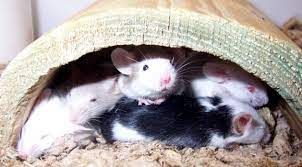
\includegraphics[width=\textwidth]{mouse}
        \caption{This is the first subcaption}
        \label{fig:a}
    \end{subfigure}
    
    \begin{subfigure}[b]{0.8\textwidth}
        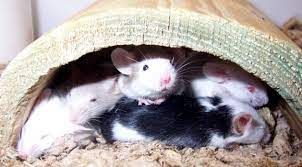
\includegraphics[width=\textwidth]{mouse}
        \caption{This is the second subcatpion}
        \label{fig:b}
    \end{subfigure}
    
    \caption{This is the overall caption}\label{fig:overall}
\end{figure}



%\bibliographystyle{plain}
\bibliographystyle{abbrv}
\bibliography{qfip_citations}
%\begin{thebibliography}{9}                                                                                                %
%\bibitem {derman_smile}Derman, E. \href{http://www.emanuelderman.com/media/smile-lecture1.pdf}
%{Lectures on Smile, Lecture 01}.
%\end{thebibliography}
\end{document}
